\documentclass{article}
\usepackage{graphicx} % Required for inserting images
\usepackage{amsmath}
\usepackage{amssymb}
\usepackage{amsthm}
\usepackage{physics}
\usepackage{unicode-math}
\usepackage{mathtools}
\usepackage{graphicx}
\usepackage[T1]{fontenc}
\usepackage{cfr-lm}
\graphicspath{ {./images/} }
\usepackage{blindtext}
\usepackage{hyperref}
\usepackage{eucal}
\usepackage{pgfplots}
\usepackage{cancel}
\usepackage{comment}
\usepackage{ textcomp }
\usepackage{fourier}

%\usepackage[letterpaper,top=2cm,bottom=2cm,left=3cm,right=3cm,marginparwidth=1.75cm]{geometry}  
\hypersetup{
    colorlinks=true,
    linkcolor=blue,
    filecolor=magenta,      
    urlcolor=cyan,
}



\title{Quantum Physics}
\author{Luigi Pagani}
\date{Academic Year 2022-2023}


\begin{document}
\maketitle
\noindent 

\section*{Release Note}
\textbf{Version 2.2 \today} \\
This document contains the lecture notes for the Quantum Physics course held at Polytechnique University of Milan during the academic year 2022-2023 by Professor Marco Finazzi. 
The most up to date version of this notes is available at this \href{https://it.overleaf.com/read/wtnwkpkkyzsq}{link}.

\section*{ \danger \  Notation}
In these notes, I use the standard bra-ket notation for quantum mechanics. However, for scalar operators, the "hat" $\hat{O}$ has been sometimes omitted to make the notation less heavy.
We also  use an abuse of notation, indeed in this notes  $\bra{v\hat{A}}$ stands for $\bra{\hat{A}v}$, and we will use them interchangeably. 

\newpage 
\tableofcontents 
\newpage
\section{Lecture 1}

Light is an electromagnetic wave, since we can observe the phenomenon of diffraction.
Even firing a single electron many times through a crystal, we do observe a diffraction lattice, thus electron is both a wave and a particle.
In this class, we will study non relativistic quantum Mechanics. Relativistic effects are negligible if the velocity of the particle is small, or in a more rigours way if: $E_k \ll E_0 = mc^2.$
Since in the quantum mechanical world we can observe diffraction phenomena, we need to build a model where the superposition principle holds. So we need a vector field. In this vector field, quantum states are called \emph{kets}, and the symbol associated to them is the following one: $ \ket{u}$.
Now we will illustrate the basic mathematical properties of kets.

\begin{itemize}

\item $\alpha \ket{u} \triangleq \ket{\alpha u}$

\item $ \ket{u} + \ket{v} \triangleq \ket{u+v}$

\item $ \bra{u} \ket{\alpha v} \triangleq \alpha \bra{u} \ket{v} $

\item $ \bra{u}\ket{v} \triangleq \bra{v}\ket{u}^*$

\item $\bra{v}\ket{n+w} \triangleq \bra{v}\ket{n} + \bra{v}\ket{w}$ 

\end{itemize}
A space satisfying all these properties is called an Hilbert Space. So Quantum States form an Hilbert Space.
The \emph{bra} is an operator associating a vector in Hilbert space to a complex scalar. The notation for the \emph{bra} is the following: $\bra{v}$. The bra space is the dual of the kets Hilbert space.
\begin{itemize}

\item  $\bra{\alpha u} \triangleq \alpha^* \bra{v}  $ 

\item $ \bra{u+v} \triangleq \bra{u} + \bra{v}$

\end{itemize}
We can define a norm: $\norm{u} = \sqrt{\bra{u}\ket{u}}\in \mathbb{R^+}$.
The norm satisfy: 
$$\norm{u+v} \leq \norm{u} + \norm{v}. $$
$$\norm{ \bra{u}\ket{v}}^2 \leq \bra{u}\ket{u}  \cdot \bra{v}\ket{v}$$

\section{Lecture 2}

Quantum states are characterised by:
\begin{itemize}
    \item Wave particle Duality
    \item  Lack of Determinism
    \item Superposition Principle
\end{itemize}
Now we introduce the concept of observables. In quantum mechanics the result of an experiment is always a real number. In quantum mechanics if you make a measurement on the same quantum state, you do not necessarily get back the same observable value. The specific quantum states which have this properties are called pure states.
For example, if I shot an electron against a detector, not passing by a slit or crystal, I always get the measurement of the electron in the same position. Pure states always exist for any observable and for any quantum state. The pure states can be used to construct our Hilbert Space. They will be the basis of the Hilbert Space, since pure states are orthogonal to each other. \\
If we have the following state $\ket{u} = \alpha \ket{n} + \beta \ket{v}$, where $\ket{n}$ and $\ket{v}$ are pure states, respectively with the associated observables $N$ and $V$, the observables we can get from measuring $\ket{u}$ is either $N$ or $V$, not a combination of the twos. We can determine the time evolution of the quantum states, but not the results of the measurement. It is not a lack of information, the randomness is intrinsic to the measurement.
We will indicate with $P(N)$ the probability of getting the observable $N$ from our measurement.
For the quantum state $\ket{u}$, the following holds true:  $P(N) = \frac{\alpha^2}{\alpha^2+\beta^2}$.\\
We can restrict the study to unitary quantum states. So, assuming that $\alpha^2 + \beta^2 = 1 $, the previous equation becomes even simpler: $P(N) = \alpha^2$.
We can multiply any quantum states by any scalar, and we obtain the same quantum state.  Even limiting ourselves to states with unitary norm, we have still a lot of choices of quantum states. 
Indeed quantum states are gauge invariant: $\ket{u} $ and $ e^{i\theta} \ket{u}$ describe the same state.\\ \\
Now we must rigorously define the definition of measurement. After a measurement the state collapses to the pure state we have just observed. If I take the same measurement twice, in an interval of time arbitrary small, we will get the same observable.
The measurement reset the system in a pure state , but anyways we cannot predict the future measurement, we just find a new initial state.

\section{Lecture 3}

In this lecture we will define an algebra of observables and pure states.\\
$\ket{u} = \alpha_1 \ket{o_1} + \alpha_2 \ket{o_2} + \dots + \alpha_j\ket{o_j} = \sum_{j \in J} \alpha_j \ket{o_j}$.
As previously mentioned we will restrict our study to quantum states with unitary norm.
The pure states $o_j, j \in J$ form an orthogonal basis of our Hilbert Space. Thus the two following properties hold:

\begin{itemize}
    \item $ \norm{o_j} = 1 \ \forall j$
    \item $\bra{o_j}\ket{o_k} = \delta_{jk}$
\end{itemize}
There is a strong analogy between the discrete and continuous case, the only difference is the summation becoming an integral. \\
$$ \ket{u} = \int \alpha(\xi)\ket{o(\xi)} d \xi $$ \\ 
$$P[O(x) \leq O \leq O(x+\delta x)] \simeq  |\alpha(x)|^2 \delta x$$ \\ 
In the following expression, $ \ket{o(x_0)}$ is a pure state, thus $\alpha(x) = \delta(x-x_0)$. \\
$$\ket{o(x_0)} = \int \alpha(x) \ket{o(x)} dx = \int \delta(x-x_0) \ket{o(x)} dx = \ket{o(x_0)} $$
\paragraph{Representation of quantum states}

   \begin{align*}
    [\mathrm{A_j}] &= \begin{bmatrix}
           \alpha_1 \\
           \alpha_2  \\
           \vdots \\
           \alpha_j
         \end{bmatrix}
  \end{align*}

  \begin{align*}
    [\mathrm{B_j}] &= \begin{bmatrix}
           \beta_1 \\
           \beta_2  \\
           \vdots \\
           \beta_j
         \end{bmatrix}
  \end{align*} 
For the sum of two quantum states we can write:
$$\ket{u} + \ket{v} = \sum_{j} \alpha_j \ket{o_j} + \sum_{j} \beta_j \ket{o_j} = \sum_{j}(\alpha_j + \beta_j) \ket{o_j}  $$
For the inner product:
  $$\bra{v}\ket{u} = \bra{ \Bigl( \sum_j \beta_j \ket{o_j} \Bigl) }\ket{ \Bigl( \sum_k{\alpha_k \ket{o_k}} \Bigl) } = \sum_{j,k} \bra{\beta_j \ket{o_j}} \ket{(\alpha_k \ket{o_k}} = \sum_{j,k} \beta^*_j \alpha_k \bra{o_j} \ket{o_k} = \sum_j \beta_j^* \alpha_j.$$
  For the continuous case, the sum become an integral, so:
  $$ \bra{v}\ket{u} = \int \beta^*(x) \alpha(x) dx$$
We can also change the basis of our Hilbert Space, to find the coefficient in two different basis:
$ \alpha_j = \bra{v_j} \ket{u}$ and $\beta_k = \bra{w_k}\ket{u}$.
I the next step we will derive the formula for the change of basis. \\ 
$1) \ \alpha_j = \bra{v_j}\ket{u}$ \\
$2)\  \ket{v_j} = \sum_k \bra{w_k} \ket{v_j} \ket{w_k}$. \\
Substituting $2)$ in $ 1)$, we obtain the following: $$\alpha_j = \sum_k \bra{w_k} \ket{v_j}^* \bra{w_k} \ket{u} = \sum_k \bra{v_j} \ket{w_k} \bra{w_k} \ket{u} = \sum_k \bra{v_j} \ket{w_k} \beta_k$$.

\section{Lecture 4}
The coefficients of a quantum state in two different bases are related by the expressions $\alpha_j = \sum_k M_{jk} \beta_k$, with $M_{jk}=\langle o_j \vert v_k \rangle$ and $\beta_k = \sum_j M_{kj}' \alpha_j$, with $M_{kj}' = \langle v_k \vert o_j \rangle$. The matrices $M$ and $M'$ are the change of basis matrix.\\ \\
If we apply the change of basis twice, back and forth, obviously $MM'= I, M'M=I$.
This condition is equivalent to saying that $M,M'$ are unitary matrices. A unitary matrix preserves the inner product and the norm of a quantum state, which means that it preserves the probabilities of measurement outcomes. Therefore, a change of basis that is represented by a unitary matrix is a valid transformation in quantum mechanics.
For the continuous case it becomes:
$$ \alpha(\xi) = \int d\chi f(\xi,\chi) \beta(\chi),$$where  $f(\xi,\chi) = \bra{o(\xi)}\ket{v(\chi)}$.\\ \\
\textbf{Operators} \\ \\
Operators are functions on Hilbert Spaces: $\mathcal{H} \mapsto \mathcal{H}$.
Now we will study the properties of the projector operator.
$\hat{P}_{oj} \triangleq \ket{o_j}\bra{oj}$.
The projector is applied to a ket: $\hat{P}_{oj}\ket{v} =\ket{o_j}\bra{oj}\ket{v}.$ \\
In quantum mechanics operators are associated to observables. If $\ket{o_j}$ are pure states and $O_j$ the associated observables, we define the operator $$\hat{O} = \sum_j O_j \ket{o_j}\bra{o_j}.$$
For continuous systems, the situation is similar:
$$\hat{O} \triangleq \int d\xi \hat{O}(\xi) \ket{o(\xi)}\bra{o(\xi)}.$$
Let's prove that $$\bra{w}  \hat{O}\ket{v}   =\bra{\hat{O}w}\ket{v} = \bra{w}  \ket{\hat{O}v} $$by explicitly expanding the sum. We know that the operator $\hat{O}$ is given by:
$$\hat{O} = \sum_j O_j \ket{o_j}\bra{o_j}$$
Now, let's compute the inner product $\bra{w} \ket{Ov}$:
$$ \bra{w}\ket{Ov}  = \bra{w} \ket{\sum_j O_j \ket{o_j}\bra{o_j} \ket{v}}$$
Using linearity of the inner product, we can expand the sum:
$$ \bra{w}\ket{\hat{O}v}   = \sum_j O_j \bra{w}  \ket{o_j}\bra{o_j} \ket{v}$$
Now, let's compute the inner product $\bra{\hat{O}w}\ket{v}$:
$$\bra{\hat{O}w}\ket{v}= \bra{ \Bigl( \sum_j O_j \ket{o_j}\bra{o_j}  \ket{w} }  \ket{v}$$
Again, using antilinearity of the inner product,the fact that $O_j \in \mathbb{R}$ and the properties of the conjugate, we can expand the sum in the following way:
$$\bra{\hat{O}w}\ket{v} = \sum_j O_j^* \bra{o_j}\ket{w}^* \bra{o_j}\ket{v} = \sum_j O_j \bra{w}\ket{oj} \bra{o_j}\ket{v}.$$
We have just shown that:
$$\bra{w}  \hat{O}\ket{v}   =\bra{\hat{O}w}\ket{v} = \bra{w}  \ket{\hat{O}v}. $$
Now we will uncover the relationship between the operator $\hat{O}$ and the ket $\ket{o_{j0}}$.
$$\hat{O} \ket{o_{j0}} = \sum_j O_j \ket{o_j} \bra{o_j}\ket{o_{j0}} = O_{j0} \ket{o_{j0}}.  $$
So pure states are the eigenstates of the operators, and the observables are the associated eigenvectors.
For a general quantum states, instead we get:
$$\hat{O} \ket{o} = \sum_j O_j \ket{o_j} \bra{o_j}\ket{o} = \sum_j O_j \alpha_j \ket{o_j}.$$

Let's introduce a new notation. $\langle O \rangle$ is the expected value of the observable.
\begin{align*}
 \langle O \rangle  = \sum_j O_j P(O_J) = \sum_j O_j  | \alpha_j |^2 = \sum_j O_j \bra{v}\ket{o_j}\bra{o_j}\ket{v} = \\ = \sum_j  \bra{v} O_j \ket{o_j} \bra{o_j}\ket{v} 
 = \bra{v} \sum_j O_j \ket{o_j}\bra{o_j}\ket{v} = \bra{v} \hat{O} \ket{v}.
 \end{align*}

\section{Lecture 5}

$$ \ket{u} = \sum_j \alpha_j \ket{o_j} \ \ \ \ \ \ket{u} = \sum_k \beta_k \ket{v_k} $$
 We can represent the same kets in two different bases. In the eigenstates bases we define the diagonal matrix associated to an operator. Let's note that $M^{-1}_{kj} = M_{jk}^*$. We can translate a vector in the two bases with the following operations:
 
   \begin{align*}
    \begin{bmatrix}
           \alpha_1 \\
           \alpha_2  \\
           \vdots \\
           \alpha_j
         \end{bmatrix}  =  \Bigr[ \mathrm{M_{kj}^{-1}} \Bigr] \begin{bmatrix}
             \beta_1 \\
             \beta_2 \\
             \vdots \\
             \beta_j
         \end{bmatrix}
  \end{align*}
If $\hat{D}$ is the operator of $\hat{O}$ in its diagonal form, the following equality holds:
  
  $$ \hat{O} =  \Bigr[M_{kj} \Bigr] \hat{D} \Bigr[ M_{kj}^{-1} \Bigr] $$
  What we have just stated is a \href{https://en.wikipedia.org/wiki/Spectral_theorem#Normal_matrices}{generalization of the spectral theorem for normal matrices}, using the property that $M$ is a unitary matrix, and thus $M^{-1} = M^{\dag}$.\\ \\
Now we will see the position operator, for a two dimensional system. 
$$ \hat{X}_0 = \begin{bmatrix}
    x_0 \ 0 \\
    0    \ -x_0 \\
\end{bmatrix}$$
with eigenstates given by $ \ket{x_0} = \begin{bmatrix}
    1 \\
    0 \\
\end{bmatrix} , \ket{-x_0} = \begin{bmatrix}
    0 \\
    1 \\
\end{bmatrix} $, with eigenvalues $l_{1/2} = \pm x_0$ \\ \\ 
Now we will define the reflection operator $\hat{R} = \begin{bmatrix}
    0 \ \ 1 \\
    1\  \ 0 \\
\end{bmatrix}$ with eigenstates: \\$ \ket{g} = \begin{bmatrix}
\frac{1}{\sqrt2} \\ \\
\frac{1}{\sqrt2}
\end{bmatrix}, \ket{u} = \begin{bmatrix}
    \frac{1}{\sqrt2} \\ \\
    -\frac{1}{\sqrt2}
\end{bmatrix}$ associated to the eigenvalues $ \lambda_1 = 1, \lambda_2 = -1$. \\  \\
$$\ket{v} = \alpha_1 \ket{x_0} + \alpha_2 \ket{-x_0}$$
$$\ket{v} = \beta_1 \ket{g} + \beta_2 \ket{u}$$ \\
Now let's explore the relationship between the two basis:\\
$$\ket{v} = \alpha_1 \ket{x_0} + \alpha_2 \ket{-x_0} \ , \
\ket{v} = \beta_1 \ket{g}  + \beta_2 \ket{u} $$ 
$$ \alpha_1 =  \bra{x_0}\ket{v} = \beta_1 \bra{x_0}\ket{g} + \beta_2 \bra{x_0}\ket{u}$$
$$ \alpha_2 =  \bra{-x_0}\ket{v} = \beta_1 \bra{-x_0}\ket{g} + \beta_2 \bra{-x_0}\ket{u}$$\\
In matrix form, the change of basis become: \\
$$ \begin{bmatrix}
    \alpha_1 \\
    \alpha_2 \\ 
\end{bmatrix} = \begin{bmatrix}
    \bra{x_0}\ket{g} \ \ \bra{x_0}\ket{u} \\
    \bra{-x_0}\ket{g} \  \ \bra{-x_0}\ket{u} \\
\end{bmatrix} \begin{bmatrix}
    \beta_1 \\
    \beta_2 \\
\end{bmatrix}$$. \\ \\
We call the newfound matrix $U = \begin{bmatrix}
    \bra{x_0}\ket{g} \ \ \bra{x_0}\ket{u} \\
    \bra{-x_0}\ket{g} \  \ \bra{-x_0}\ket{u} \\
\end{bmatrix} $
$$\hat{X}_p = U^{-1} \hat{X}_x U = \begin{bmatrix}
    0 \ x_0 \\
    x_0 \ 0 \\
\end{bmatrix}$$ 
The position operator in parity form has obviously the same eigenstates of the reflection one.
Now let's define $\hat{H}$, the Hamiltonian operator, which gives us the total energy of the system.
$\hat{R}$ is the reflection operator:
$$\hat{R} = \begin{bmatrix}
    0 \ 1 \\
    1 \ 0 \\
\end{bmatrix}$$
$$\hat{H} \ket{e} = E \ket{e}$$
We are assuming to be working on the Ammonia molecule, which can be rotated around its axis passing vertically through the Nitrogen.\\ \\
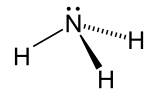
\includegraphics[scale = 0.75]{ammonia.png} \\ \\
For physical reason, rotating the systems should not change its energy level, thus we impose the following constraint:
$$ \hat{H}\hat{R}\ket{e} = E\hat{R}\ket{e}  \implies
\hat{R}\hat{H}\hat{R}\ket{e} = E\hat{R}\hat{R}\ket{e} = E\ket{e} = \hat{H}\ket{e}.$$
Thus $\hat{R}\hat{H}\hat{R} = \hat{H}$.
Since the operators are Hermitian, $\hat{H}$ has the following form:
$$\hat{H} = \begin{bmatrix}
    a \ b \\
    b^* \ c \\
\end{bmatrix}$$
If we impose the previous condition, we get that the matrix has indeed the following form:
$$\hat{H} = \begin{bmatrix}
    a \ b \\
    b \ a \\
\end{bmatrix}$$
The eigenvalues of $\hat{H}$ are $\lambda =  a \pm b$. If we impose $a=0$, since energy is defined up to a constant, we get that $E = \pm b = \pm \frac{\Delta E}{2}$. \\
Thus we get: $$\hat{H} = \begin{bmatrix}
    0 \ \ \frac{\Delta E}{2} \\ \\
    \frac{\Delta E}{2} \ \ 0    \\
\end{bmatrix}$$ 
In the fundamental state, the energy will occupy the lowest energy state, so $E = - \frac{\Delta E}{2}$, assuming $\Delta E > 0.$ The eigenstate associated with this eigenvalue is $\ket{g}$, the parity eigenstate.
The expected value of the position is obviously 0. 
$$ \langle X \rangle = \bra{g} \hat{X} \ket{g} = 0. $$

\section{Lecture 6}

Now we will find out the form of the velocity $\hat{V}$ operator. The most general form of an Hermitian operator is the following one:
$$\hat{V} = \begin{bmatrix}
    a \  b \\
    b^* \ c \\
\end{bmatrix} \  \ a,c \in \mathbb{R}, b \in \mathbb{C}. $$

If $\hat{V} \begin{bmatrix}
    \alpha_1 \\
    \alpha_2 \\
\end{bmatrix} = v \begin{bmatrix}
    \alpha_1 \\
    \alpha_2 \\
\end{bmatrix}$, then:
$$\hat{V} \hat{R} \begin{bmatrix}
    \alpha_1 \\
    \alpha_2 \\
\end{bmatrix} = -v \hat{R}\begin{bmatrix}
    \alpha_1 \\
    \alpha_2 \\
\end{bmatrix} \implies \hat{R}\hat{V}\hat{R}\begin{bmatrix}
    \alpha_1 \\
    \alpha_2 \\
\end{bmatrix} = -v \begin{bmatrix}
    \alpha_1 \\
    \alpha_2 \\
\end{bmatrix} \implies \hat{R}\hat{V}\hat{R} = - \hat{V}$$
Solving this equations, we obtain the constraints on the operator:
$$\begin{cases}
     &  c=-a \\
     & b =-b^*\\ 
\end{cases} $$
Thus $b$ is a pure complex number. We can write the matrix $\hat{V}$ in the following simplified form: \ \ 
$$\hat{V} = \begin{bmatrix}
    a \ \ id  \\
    -id \ \ -a \\
\end{bmatrix}  \ \ a,d \in \mathbb{R}$$
The eigenvalues of $\hat{V}$ are: $v= \pm \sqrt{a^2+d^2}$.
For the Heisenberg uncertainty principle, $d \neq 0$. If $d = 0$, then $\hat{V}$ and $\hat{X}$ would have the same eigenstates, thus in those two states we would know with certainty both the position and the velocity.\\  \\
\textbf{Qubits} \\
Now we will introduce the notion of Qubits, which is the name for a quantum system with two basis vectors. \\ 
We introduce the following notation for the basis vectors: $\ket{0}, \ket{1}$.
$\ket{v} = a\ket{0}+b\ket{1} $, with the constraints that $\norm{a}^2+\norm{b}^2=1.$\\
Since quantum systems are gauge invariant, we can write:
$$ \ket{v} = z\ket{0}+ (x+iy) \ket{1} \ , \ x,y,z \in \mathbb{R}.$$
We can rewrite the following expression: \\
$ z = cos \bigl( \frac{\theta}{2} \bigl) $\\
$ x +iy = e^{i\phi}sin\bigl( \frac{\theta}{2} \bigl)$
\\
Any Hermitian matrix has the following form:
$$\hat{O} = \begin{bmatrix}
    \delta +\alpha \ \ \  \gamma-i\beta \\
    \gamma + i\beta \ \ \  \delta - \alpha \\ 
\end{bmatrix} \ , \ \alpha,\beta,\gamma, \delta \in \mathbb{R}$$
We can decompose the generic operator $\hat{O} = \alpha \hat{\sigma}_z + \beta \hat{\sigma}_y + \gamma \hat{\sigma}_x + \delta \hat{I} $ with the Pauli matrices.

$$\hat{\sigma}_x = \begin{bmatrix}
    0 \ \  1 \\ 1 \ \ 0
\end{bmatrix} \ , \ \hat{\sigma}_y =\begin{bmatrix}
    0 \ \ -i \\ i \  \ 0
\end{bmatrix} \ , \ \hat{\sigma}_z = \begin{bmatrix}
    1 \ \  0 \\ 0 \ \ -1
\end{bmatrix} $$
Each of these Pauli matrices represent a $180$° rotation around the $x,y,z$ axis of the Bloch Sphere. Any rotation around the axis can indeed be represented as a linear combination of the identity operator and one of the Pauli matrices.
$$\hat{R}_x(\theta)= cos\biggl(\frac{\theta}{2} \biggl) \hat{I} - i sin \biggl(\frac{\theta}{2} \biggl) \hat{\sigma_x}.$$
The equations is analogous for the other two axis.
$$\hat{R}_y(\theta)= cos\biggl(\frac{\theta}{2} \biggl) \hat{I} - i sin \biggl(\frac{\theta}{2} \biggl) \hat{\sigma_y}.$$
$$\hat{R}_z(\theta)= cos\biggl(\frac{\theta}{2} \biggl) \hat{I} - i sin \biggl(\frac{\theta}{2} \biggl) \hat{\sigma_z}.$$
\\ \\ 
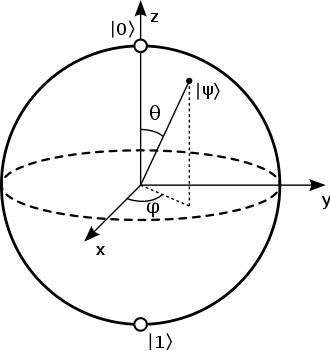
\includegraphics[scale=0.6]{Bloch_sphere.svg.png} \\ \\  \\ 
Let's close this little introduction to qubits, and review the Hamiltonian operator: 
$$\hat{H}\ket{u} = E\ket{u} \implies \hat{H}\hat{R} \ket{u} = E\hat{R}\ket{u} \implies \hat{R}^{-1} \hat{H}\hat{R} = E \hat{R}^{-1}\hat{R}\ket{u} = E\ket{u} = \hat{H} \ket{u}.$$
$$\implies \hat{R}^{-1}\hat{H}\hat{R}=\hat{H} \implies \hat{H}\hat{R} = \hat{R}\hat{H}. $$
We have just proved that $\hat{H}$ and $\hat{R}$ commute.
$$\hat{H}\hat{R}\ket{v}=\hat{R}\hat{H}\ket{v} \implies \hat{H}p\ket{v} = \hat{R}\hat{H}\ket{v},$$
where $p$ is the parity, such that: $p\ket{u} = \hat{R}\ket{u}.$ \\  \\
\textbf{Theorem}\\
Two Hermitian operators commute if and only if they have a common eigenbasis. \\ \\
I will prove it with the hypothesis that all the eigenvectors are non degenerates.  This theorem also holds true when without this hypothesis, but it is more complicated to prove. The more complete version of the proof is available at this
\href{https://ocw.mit.edu/courses/8-04-quantum-physics-i-spring-2013/9ccc9fd132124dd102e1a7863e6e12ce_MIT8_04S13_OnCommEigenbas.pdf#page=3}{link}.
\\ \\
\begin{comment}
As we have seen in the last lecture:
$$p\ket{u}=\hat{R}\ket{u}$$
$$\ket{u} = \alpha \ket{v}$$
$$\hat{H}\ket{v} = \alpha \ket{v}$$ 
$$\ket{u} = \sum_k \alpha_j \ket{v_j}$$\\ 
\end{comment}
$\implies$ Starting from $A\ket{v_j}=\lambda{v_j}$, we have:
$$AB\ket{v_j} = BA\ket{v_j} = B \lambda \ket{v_j} = \lambda B\ket{v_j}$$
Thus $\ket{v_j}$ and $B\ket{v_J}$ are both eigenvectors of $A$, sharing the same $\lambda$. Since  $A$ is Hermitian, and thus diagonalizable, its eigenvectors are distinct, the eigenspaces are one dimensional, then $B\ket{v}$ must be a multiple of $\ket{v}$. In other words $\ket{v}$ is an eigenvector of $B$ as well as $A$.\\ \\
$\impliedby$ Since $A$ and $B$ have a common eigenbasis identified by $\ket{v}_j \in J$ 
$$\hat{A}\ket{v_j} = \alpha_j \ket{v}$$ 
$$\hat{B}\ket{v_j} = \beta_j \ket{v}$$ 
$$ \hat{A}\hat{B} \ket{u} = \sum_j \alpha_j \hat{A}\hat{B} \ket{v_j} = \sum_j \alpha_j \hat{A} b_j \ket{v_j} =  \sum_j \alpha_j  b_j \hat{A} \ket{v_j} = \sum_j \alpha_j b_j a_j \ket{v_j}. $$ \\ 
$$\hat{B}\hat{A}\ket{u}= \sum_j \alpha_j \hat{B}\hat{A}\ket{v_j} = \sum_j \alpha_j \hat{B}a_j \ket{v_j} = \sum_j \alpha_j a_j \hat{B}\ket{v_j} = \sum_j \alpha_j a_j b_j \ket{v_j} \ \blacksquare$$


\section{Lecture 7}
If $\hat{A}\hat{B} \neq \hat{B}\hat{A} \implies \hat{A}\hat{B} - \hat{B}\hat{A} \neq 0.$
We define the commutator operator:$$ \bigl[\hat{A},\hat{B} \bigl] = \hat{A}\hat{B} - \hat{B}\hat{A}.$$ 
We define the also variance of an operator: 
\begin{align*}
   \sigma^2 \triangleq \sum_j \bigl( O_j -\langle o \rangle \bigl)^2 P \bigl(O_j\bigl) = \bra{v} \bigl( \hat{O} - \langle o \rangle \bigl)^2 \ket{v}   = \bra{v} \hat{O}^2 \ket{v} + \langle o \rangle^2 -2 \langle o \rangle \bra{v} \hat{O} \ket{v} = \\ = \bra{v} \hat{O}^2 \ket{v} + \langle o \rangle^2 -2 \langle o \rangle^2 =  \bra{v} \hat{O}^2 \ket{v} - \langle o \rangle^2 = \bra{v} \hat{O}^2 - \langle o \rangle^2 \ket{v} \hspace{2 cm}.
\end{align*}
We have used the notation that $\langle o \rangle = \bra{v}\hat{O}\ket{v}$.\\
Moreover, let's verify that he first two definitions are equivalent, since:
$$\sigma^2 = \sum_j \biggl(O_j - \langle o \rangle\biggl)^2 P(O_j) = \sum_j \bigl(O_j^2-2O_j\langle o \rangle + \langle o \rangle^2 \bigl) P(O_j)=$$
$$= \sum_j O_j^2P(O_j)- \langle o \rangle^2 = \bra{v}\hat{O}^2\ket{v}-\langle o \rangle^2 = \bra{v}\hat{O}^2-\langle o \rangle^2 \ket{v}.$$
Now we will define the following operator:
$$\hat{A'} = \hat{A} - \langle A \rangle.$$
On Hilbert Spaces the Cauchy-Schwartz Inequality holds:
$$ \norm{\bra{u}\ket{w}}^2 \leq \bra{u}\ket{u}\bra{w}\ket{w}. $$
For the operators $\hat{A}, \hat{B}$, exploiting the Hermitian property, in the same way
as the formula for the computation of the variance$ \biggl( \mathrm{Var}(X) = \mathrm{E}[(X - \mathrm{E}(X))^2] = \mathrm{E}(X^2) - [\mathrm{E}(X)]^2 \biggl)$, we can write:
$$\sigma_A^2 =  \bra{v} \hat{A}^2 - \langle A \rangle ^2 \ket{v} = \bra{v} \hat{A'}^2 \ket{v}= \bra{v \hat{A'}} \ket{\hat{A'} v}$$
$$\sigma_B^2 =  \bra{v} \hat{B}^2 - \langle B \rangle ^2 \ket{v} = \bra{v} \hat{B'}^2 \ket{v}= \bra{v \hat{B'}} \ket{\hat{B'} v}$$ 
We can now apply the CS Inequality, with $\ket{u} = \hat{A'}\ket{v}$ and $ \ket{w} = \hat{B'}\ket{v}.$
\begin{gather*}
  \sigma_A^2\sigma_B^2 \geq  \norm{\bra{v \hat{A'}}\ket{\hat{B}'v} }^2 \triangleq \norm{ \bra{v} \hat{A'}\hat{B'}\ket{v}}^2 \geq  Im \bigl( \bra{v}\hat{A'}\hat{B'} \ket{v} \bigl)^2 = \\ = \frac{1}{4} \norm{ \bra{v}\hat{A'}\hat{B'}\ket{v} - \bra{v}\hat{A'}\hat{B'}\ket{v}^* }^2 
  =\frac{1}{4} \norm{ \bra{v}\hat{A'}\hat{B'}\ket{v} - \bra{v}\hat{B'}^\dag \hat{A'}^\dag \ket{v} }^2= \\ = \frac{1}{4} \norm{ \bra{v}\hat{A'}\hat{B'}\ket{v} - \bra{v}\hat{B'}\hat{A'}\ket{v} }^2  =  \frac{1}{4} \norm{ \bra{v}\hat{A'}\hat{B'} - \hat{B'}\hat{A'}\ket{v} }^2 =\frac{1}{4} \norm{ \bra{v} [\hat{A'},\hat{B'}]\ket{v} }^2 \\ \implies \sigma_A^2\sigma_B^2 \geq   \frac{1}{4} \norm{[\hat{A'},\hat{B'}] }^2 =\frac{1}{4} \norm{ \bra{v} [\hat{A'},\hat{B'}]\ket{v} }^2 \\ \implies \sigma_A^2\sigma_B^2 \geq   \frac{1}{4} \norm{[\hat{A'},\hat{B'}] }^2  . 
\end{gather*}
Applying this formula to the Position and Hamiltonian Operator and the ket $\ket{v} =\Bigl[ \frac{1}{\sqrt{2}} -\frac{i}{\sqrt{2}} \Bigl] $ we get:
$$ \sigma_x \sigma_E \geq \frac{1}{2} \norm{ \bra{v} [\hat{X'},\hat{H'}]\ket{v} } = \frac{1}{2} xo \Delta E$$
$$ \sigma_x^2 = \bra{v} \hat{X}^2 - \langle x \rangle \ket{v} = \bra{v} \hat{X}^2 \ket{v} - \langle x \rangle^2 = x_0^2$$
$$\sigma_E^2 = \bra{v} \hat{H}^2 - \langle E \rangle ^2 \ket{v} = \bra{v} \hat{H}^2 \ket{v} - \langle E \rangle ^2 = \frac{\Delta E^2}{4}$$

\paragraph{Composites Systems}In a composite system, there are new degrees of freedom. For example the position of the two Hydrogen atoms in the H2-TPP. \\ \\

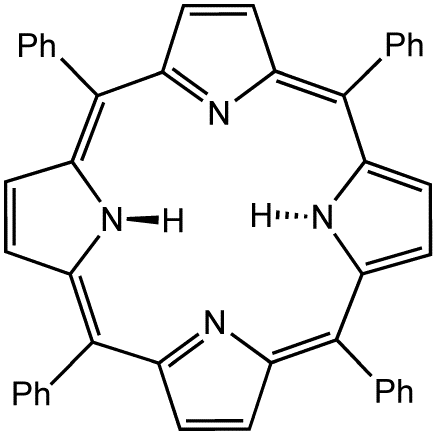
\includegraphics[]{H2TPP.png}
\\ \\
$$\mathcal{H}_x \mapsto \ket{u^{(x)}} \ ,\ \ \mathcal{H}_y \mapsto \ket{u^{(y)}}$$

$$ \ket{u^{(x)}u^{(y)}} \triangleq \Bigl( \ket{u^{(x)}} \Bigl) \Bigl( \ket{u^{(y)}} \Bigl) \in \mathcal{H}_x \otimes \mathcal{H}_y.$$ \\
The Tensor product of Hilbert Spaces is still an Hilbert Space. 

$$ \Bigl( \ket{u^{(x)} + v^{(x)}} \Bigl) \Bigl( \ket{u^{(y)}+ v^{(y)}} \Bigl) \triangleq \ket{u^{(x)} u^{(y)}} + \ket{v^{(x)}v^{(y)}} + \ket{u^{(x)}v^{(y)}}+\ket{v^{(x)}u^{(y)}}.$$

$$\bra{v^{(x)} v^{(y)}} \ket{{u^{(x)}u^{(y)}}} \triangleq \bra{v^{(x)}}\ket{u^{(x)}} \bra{v^{(y)}}\ket{u^{(y)}}.$$

If: $$\hat{O}^{(x)} \ket{u^{(x)}} = \ket{w^{(x)}} \implies \hat{O}^{(x)} \ket{u^{(x)}v^{(y)}} = \ket{w^{(x)}v^{(y)}}.$$
Let's introduce more definitions and equality:
$$\hat{O}^{(x)}\hat{O}^{(y)}\ket{u^{(x)}u^{(y)}} \triangleq \ket{w^{(x)}w^{(y)}} \triangleq \hat{O}^{(y)}\hat{O}^{(x)}$$

$$\ket{u^{(x)}} = \sum_j \alpha_j^{(x)} \ket{o_j^{(x)}}$$
$$\ket{u^{(y)}} = \sum_k \beta_k^{(u)} \ket{o_j^{(u)}} $$
$$\ket{u^{(x)}u^{(y)}} = \sum_{jk} \alpha_j^{(x)}\beta_k^{(y)} \ket{o_j^{(x)}o_k^{(y)}}$$

\section{ Lecture 8}
Energy of the H2-TPP. Four degrees of freedom.
$$\ket{x} \mapsto \begin{bmatrix}
    \alpha_1 \\
    \alpha_2 \\
\end{bmatrix} \ , \ \ket{y} \mapsto \begin{bmatrix}
    \beta_1 \\
    \beta_2 \\
\end{bmatrix}$$

$$\implies \ket{xy} \mapsto \Biggl\{ \begin{bmatrix}
    \alpha_1 \\
    \alpha_2 \\
\end{bmatrix}_x, \begin{bmatrix}
    \beta_1 \\
    \beta_2 \\
\end{bmatrix}_y \Biggl\}$$
To find the eigenstates, we impose the condition that: 
\begin{align*} 
\begin{bmatrix}
    0 \ \frac{\Delta E}{2} \\
    \frac{\Delta E}{2} \ 0 \\
\end{bmatrix}_x \cdot \ \Biggl\{ \begin{bmatrix}
    \alpha_1 \\
    \alpha_2 \\
\end{bmatrix}_x,\begin{bmatrix}
    \beta_1 \\
    \beta_2 \\
\end{bmatrix}_y \Biggl\} \ + \begin{bmatrix}
    0 \ \frac{\Delta E}{2} \\
    \frac{\Delta E}{2} \ 0 \\
\end{bmatrix}_y \cdot \ \Biggl\{ \begin{bmatrix}
    \alpha_1 \\
    \alpha_2 \\
\end{bmatrix}_x,\begin{bmatrix}
    \beta_1 \\
    \beta_2 \\
\end{bmatrix}_y \Biggl\} = \\ \\ = \frac{\Delta E}{2}  \Biggl\{ \begin{bmatrix}
    \alpha_2 \\
    \alpha_1 \\
\end{bmatrix},\begin{bmatrix}
    \beta_1 \\
    \beta_2 \\
\end{bmatrix} \Biggl\} + \frac{\Delta E}{2} \Biggl\{ \begin{bmatrix}
    \alpha_1 \\
    \alpha_2 \\
\end{bmatrix},\begin{bmatrix}
    \beta_2 \\
    \beta_1 \\
\end{bmatrix} \Biggl\} =  \bigl(1\bigl)
\end{align*}
Assuming that $\frac{\Delta E}{2} \begin{bmatrix}
    \alpha_2 \\
    \alpha_1 \\
\end{bmatrix} = c \begin{bmatrix}
    \alpha_1 \\
    \alpha_2 \\
\end{bmatrix}$ and $\frac{\Delta E}{2} \begin{bmatrix}
    \beta_2 \\
    \beta_1 \\
\end{bmatrix} = c' \begin{bmatrix}
    \beta_1 \\
    \beta_2 \\
\end{bmatrix}$:

$$ \implies c = \pm \frac{\Delta E}{2}, \ c' = \pm \frac{\Delta E}{2}.$$

\begin{align*}
    \bigl(1\bigl) =\pm \frac{\Delta E}{2} \Biggl\{ \begin{bmatrix}
    \alpha_1 \\
    \alpha_2 \\
\end{bmatrix},\begin{bmatrix}
    \beta_1 \\
    \beta_2 \\
\end{bmatrix}  \Biggl\} \pm \frac{\Delta E}{2} \Biggl\{ \begin{bmatrix}
    \alpha_1 \\
    \alpha_2 \\
\end{bmatrix},\begin{bmatrix}
    \beta_1 \\
    \beta_2 \\
\end{bmatrix} \Biggl\} = E \Biggl\{ \begin{bmatrix}
    \alpha_1 \\
    \alpha_2 \\
\end{bmatrix},\begin{bmatrix}
    \beta_1 \\
    \beta_2 \\
\end{bmatrix} \Biggl\} \implies E = \pm \frac{\Delta E}{2} \pm \frac{\Delta E}{2}.
\end{align*}
We have just solved the eigenvalue problem. The eigenvectors are:
$$ \ket{v} = \Biggl\{ \begin{bmatrix}
     \frac{1}{\sqrt{2}} \\
    \pm \frac{1}{\sqrt{2}} \\ 
\end{bmatrix}, \begin{bmatrix}
     \frac{1}{\sqrt{2}} \\
    \pm \frac{1}{\sqrt{2}} \\ 
\end{bmatrix} \Biggl\}
$$
Let's consider a basis: $ \ket{x_0,y_0}, \ket{x_0, -y_0}, \ket{-x_0,y_0}, \ket{-x_0,-y_0}$.
 $$\Biggl\{ \begin{bmatrix}
    \alpha_1 \\
    \alpha_2 \\
\end{bmatrix},\begin{bmatrix}
    \beta_1 \\
    \beta_2 \\
\end{bmatrix} \Biggl\} \mapsto \begin{bmatrix}
    \alpha_1 \beta_1 \\
    \alpha_1 \beta_2 \\
    \alpha_2 \beta_1 \\ 
    \alpha_2 \beta_2 \\
\end{bmatrix}$$
The vector we got is still a normalized vector.

$$ \hat{H} \begin{bmatrix}
    \alpha_1 \beta_1 \\
    \alpha_1 \beta_2 \\
    \alpha_2 \beta_1 \\ 
    \alpha_2 \beta_2 \\
\end{bmatrix} = \frac{\Delta E}{2} \begin{bmatrix}
    \alpha_2 \beta_1 \\
    \alpha_2 \beta_2 \\
    \alpha_1 \beta_1 \\ 
    \alpha_1 \beta_2 \\
\end{bmatrix} + \frac{\Delta E}{2} \begin{bmatrix}
    \alpha_1 \beta_2 \\
    \alpha_1 \beta_1 \\
    \alpha_2 \beta_2 \\ 
    \alpha_2 \beta_1 \\
\end{bmatrix}  = \frac{\Delta E}{2} \begin{bmatrix}
    \alpha_2 \beta_1 + \alpha_1 \beta_2 \\
    \alpha_2 \beta_2 + \alpha_1 \beta_1 \\
    \alpha_1 \beta_1 + \alpha_2 \beta_2 \\ 
    \alpha_1 \beta_2 + \alpha_2 \beta_1 \\
\end{bmatrix}$$

$$\implies \hat{H} = \frac{\Delta E}{2} \begin{bmatrix}
    0 \ 1 \ 1 \ 0 \\
    1 \ 0 \ 0 \ 1 \\
    1 \ 0 \ 0 \ 1 \\
    0 \ 1 \ 1 \ 0 \\ 
\end{bmatrix}$$
\\
This system is analogous to two non interacting qubits.
If we want to introduce an interaction, let's study the $H_{2}$ molecule. We assume to have the following basis:
$\ket{x_0^{(1)},x_0^{(2)}},\ket{-x_0^{(1)},x_0^{(2)}},\ket{x_0^{(1)}, -x_0^{(2)}}, \ket{-x_0^{(1)} -x_0^{(2)}}.$
Let's calculate the expected value of the energy of the first and last element of the basis:
$$\bra{x_0^{(1)},x_0^{(2)}} \hat{H} \ket{x_0^{(1)},x_0^{(2)}} = \hat{H}_{11}$$
$$\bra{-x_0^{(1)},-x_0^{(2)}} \hat{H} \ket{-x_0^{(1)},-x_0^{(2)}} = \hat{H}_{44}.$$
Since having  two electrons on the same atoms costs more energy, our model doesn't consider the interaction between the electrons.
In order to have a more realistic model we need a different Hamiltonian:
$$ \hat{H} =  \begin{bmatrix}
    \alpha \ 1 \ 1 \ 0 \\
    1 \ 0 \ 0 \ 1 \\
    1 \ 0 \ 0 \ 1 \\
    0 \ 1 \ 1 \ \alpha \\ 
\end{bmatrix} $$
We get a two degrees of freedom model, with models not decoupled from each other, in order to have a more realistic model. That's the same situation of two interacting qubits.
\paragraph{Continuous Systems}

$$\ket{u} = \int \psi(\xi') \ket{\xi'} d\xi'$$
$$\bra{\xi}\ket{u} = \int \psi (\xi') \bra{\xi}\ket{\xi'}d\xi' = \int \psi (\xi') \delta(\xi -\xi') d\xi' =\psi(\xi).$$
The most natural coordinates to use is position. $\psi(x)$ is called the wave function and
$|\psi(x)|^2$ represents the probability density function.
$$P(x_0 \leq x \leq x_0 + dx) \simeq | \psi(x_0) |^2$$
Now we introduce again the position operator:
$$\langle x \rangle = \int \psi^* ( \hat{X} \psi)$$
$$ \langle x \rangle  = \int x | \psi(x) | ^2 dx = \int \psi(x)^* x \psi(x) dx.$$
Thus: $\hat{X} = x$. In the 3d space instead we get: $ \hat{\vec{r}} = \vec{r} = x \vec{u_x} + y \vec{u_y} + z \vec{u_z}. $
Now we introduce another operator, not related to an observable. The state translation operator.
$$\hat{T}_{\vec{R}} \psi(\vec{r}) = \psi(\vec{r}-\vec{R}).$$
$$\hat{T}_{\vec{R_1}}\hat{T}_{\vec{R_2}} = \hat{T}_{\vec{R_2}}\hat{T}_{\vec{R_1}} = \hat{T}_{\vec{R_1}+ \vec{R_2}}$$
Let's find the eigenstates. We can write:
$$\hat{T}_{\vec{R}} \psi(\vec{r}) = \psi(\vec{r}-\vec{R}) = \alpha_{\vec{R}} \psi(\vec{r}) \implies |\alpha_{\vec{R}}|^2 = 1.$$

$$\hat{T}_{\vec{R_1}} \psi(\vec{r}) = \alpha_{\vec{R_1}} \psi(\vec{r})$$

$$\hat{T}_{\vec{R_2}} \psi(\vec{r}) =  \alpha_{\vec{R_2}}\psi(\vec{r})$$

$$ \hat{T}_{\vec{R_1} + \vec{R_2} } \psi(\vec{r}) = \alpha_{\vec{R_1} + \vec{R_2}} \psi(\vec{r}) $$

$$\hat{T}_{\vec{R_1} + \vec{R_2}} \psi(x) = \hat{T}_{\vec{R_1}}\hat{T}_{\vec{R_2}} \psi(\vec{r}) =\alpha_{\vec{R_1}} \alpha_{\vec{R_2}}\psi(\vec{r})  \implies \alpha_{\vec{R_1}} \alpha_{\vec{R_2}} = \alpha_{\vec{R_1} + \vec{R_2}} \psi(\vec{r}) \implies \alpha_{\vec{R}} = e^{-i\vec{k} \cdot \vec{R}} $$
The associated wave function is:
$$\psi(\vec{r}) = \frac{1}{\sqrt{v}} e^{i\vec{k} \cdot \vec{r}}$$

\section{Lecture 9}

$$ \int_{\infty} \bigl| \psi(\vec{r}) \bigl| d\vec{r} = \int_{\infty} \bigl| \psi(\vec{r}-\vec{R}) \bigl|^2 d\vec{r} = \int_{\infty} \bigl| \alpha(\vec{r}) \bigl| ^2 \bigl| \psi(\vec{r}) \bigl|^2 d\vec(r) \implies \bigl| \alpha(\vec{R}) \bigl|^2 = 1. $$
This result combined with the fact that: $ \alpha(\vec{R}) = e^{-i \vec{k} \cdot \vec{R}} $ implies that $k_x,k_y,k_z \in \mathbb{R}.$
Now:
$$ \hat{T}_{\vec{R}} \psi(\vec(r)) = \alpha(\vec{R}) \psi(\vec{r}) = e^{-i \vec{k} \cdot \vec{R}} \psi(\vec{r}) = \psi(\vec{r}-\vec{R}) \implies \psi(\vec{r}) = \psi(\vec{r}-\vec{R}) e^{i \vec{k} \cdot \vec{R}} $$
Now let's introduce a new function:
$$\phi(\vec{r}) = e^{-i \vec{k} \cdot \vec{r}} \psi(\vec{r}) = e^{-i \vec{k}\cdot(\vec{r}-\vec{R})} \psi(\vec{r}-\vec{R}) = \phi(\vec{r}-\vec{R}) \ \ \forall \vec{R}.$$
$$\implies \phi(\vec{r}) = c \implies \psi(\vec{r}) = c e^{i\vec{k} \cdot \vec{r}}$$
$$\int \Bigl|c\bigl|^2 d\vec{r} =1 \implies c = \frac{1}{\sqrt{V}}.$$
We can interpret the shift by $\vec{R}$ as a change of coordinate, which leaves velocity unchanged.
$$ \vec{r} \ ' = \vec{r} -\vec{R} \implies \frac{d\vec{r} \ ' }{dt} = \frac{d\vec{r}}{dt} - \frac{d\vec{R}}{dt}  = \frac{d\vec{r}}{dt} - 0 \implies v' = v.$$
$$\hat{\vec{V}}\psi(\vec{r}) = \vec{v}\psi(\vec{r})$$
$$\hat{V}\hat{T}_{\vec{R}}\psi(\vec{r}) = \vec{v}\hat{T}_{\vec{R}}\psi(\vec{r}) = \hat{T}_{\vec{R}}\vec{v} \psi(\vec{r}) = \hat{T}_{\vec{R}}\hat{V}\psi(\vec{r}) \implies \hat{V}\hat{T}_{\vec{R}} =   \hat{T}_{\vec{R}}\hat{V}  \ \ \ \forall \vec{R} $$
For velocity and momentum we can write:
$$ \hat{V} ce^{i\vec{k} \cdot \vec{r}}=c\vec{v}e^{i\vec{k} \cdot \vec{r}}$$
For a combined system of two non interacting particles, $\vec{r_1},\vec{r_2}$, we get a wave function which is the product of the single wave functions. We will ignore the normalization factor, assuming thus that our laboratory has volume $v=1$ :
$$\psi(\vec{r_1},\vec{r_2}) = e^{i(\vec{k_1}\cdot\vec{r_1}+\vec{k_2}\cdot \vec{r_2})}$$
We impose that the total momentum of two particles, is the sum of the momentum of the isolated particles:
$$\vec{p}_1 = \vec{p}(\vec{k}_1) \ , \ \vec{p}_2 = \vec{p}(\vec{k}_2) \ , \ \vec{p}_{TOT} = \vec{p}(\vec{k}_1+\vec{k}_2) \implies \vec{p}(\vec{k}_1+\vec{k}_2) = \vec{p}(\vec{k}_1) + \vec{p}(\vec{k}_2). $$ 
That implies that: $\vec{p} \varpropto \vec{k}$, in particular $\vec{p} = \hslash \vec{k}$ 
And applying a translation in a combined system we get:
$$\hat{T}_{R}\psi(\vec{r_1},\vec{r_2}) = e^{i(\vec{k_1}\cdot\vec{r_1}-\vec{k_1}\cdot\vec{R}+\vec{k_2}\cdot\vec{r_2}-\vec{k_2}\cdot\vec{R})} = e^{-i(\vec{k_1}+\vec{k_2})\cdot\vec{R}} e^{i(\vec{k_1}\cdot\vec{r_1}+\vec{k_2}\cdot\vec{r_2})}.$$
$$\hat{T}_{R} \psi(\vec{r_1}) = e^{-\vec{k_1}\cdot \vec{R}}e^{i\vec{k_1}\vec{r_1}}.$$
$$\hat{T}_{R} \psi(\vec{r_2}) = e^{-\vec{k_2}\vec{R}}e^{i\vec{k_2} \cdot\vec{r_2}}.$$

$$\hat{P}e^{i\vec{k}\vec{r}}= \hslash \vec{k}e^{i\vec{k}\cdot\vec{r}}  =  -i \hslash \nabla  $$
$$\hat{\vec{V}} = \frac{-i\hslash}{m} \nabla $$
$\hat{\vec{P}}$ is hermitian, since all the components are Hermitian. Now let's prove it for the $x$ component.
Statement:
$$ \bra{\varphi} \hat{p}_x \ket{\psi} = \bra{\varphi} \ket{\hat{p}_x \psi} = \bra{ \varphi \hat{p}} \ket{\psi} = \bra{\hat{p}\varphi}\ket{\psi}.$$
Proof:
\begin{align*}
 \int_{-\infty}^{+\infty} \varphi^* \hat{p}_x \psi dx = -i\hslash \int_{-\infty}^{+\infty} \varphi^* \frac{\partial}{\partial{x}} \psi dx = \Bigl[ -i\hslash\varphi^*\psi \Bigl]_{-\infty}^{+\infty} + i \hslash \int_{-\infty}^{+\infty} \frac{\partial \varphi^*}{\partial x} \psi dx = \\ = 0 + \int_{-\infty}^{+\infty} i \hslash \frac{\partial \varphi^*}{\partial x} \psi dx = \int_{-\infty}^{+\infty} \bigl( \hat{p}_x \varphi \bigl)^* \psi dx =  \end{align*}
The first  definite integral is zero, because we are talking about density functions, its absolute value integrated over the entire space must be finite, so the function goes to zero at infinity. In the last step, it was used the fact that the product of the complex conjugate is the complex conjugate of the product.

\paragraph{The Heisenberg Uncertainty Principle}
\begin{gather*}
    \sigma_x\sigma_{px} \geq \frac{1}{2} \bigl| \bra{\varphi} [ \hat{X}, \hat{P}_x] \ket{\varphi} \bigl| = \frac{1}{2} \biggl| \bra{\varphi} \hat{x}\hat{p}_x - \hat{p}_x \hat{x} \ket{\varphi} \biggl| = \frac{1}{2} \biggl| \int \varphi^* (\hat{x}\hat{p}_x -\hat{p}_x\hat{x}) \varphi dx \biggl| = \\ =  \frac{1}{2} \biggl| -i\hslash \int \biggl[\varphi^* x \frac{\partial \varphi}{\partial x} - \varphi^* \frac{\partial{(x\varphi)}}{\partial x} \biggl] dx \biggl|  = \frac{\hslash}{2} \biggl| \int \biggl\{ \varphi^* x \frac{\partial \varphi}{\partial x} - \varphi^* \biggl[ x \biggl( \frac{\partial \varphi}{\partial x} + \varphi \biggl)\biggr] \biggr\} dx \biggr| = \\ = \frac{\hslash}{2} \Biggl| \int \varphi^* \varphi dx \Biggl|= \frac{\hslash}{2} \\ 
    \implies \sigma_x\sigma_{px} \geq \frac{\hslash}{2}  .
\end{gather*}
\section{Lecture 10}
\textbf{Continuous Systems in Momentum Representation}\\
Let's remember that here $\ket{\vec{r}},\ket{\vec{p}}$ are respectively position and momentum eigenstates.
$$\psi(\vec{r}) \triangleq \bra{\vec{r}}\ket{u}$$
$$\Psi(\vec{p}) \triangleq \bra{\vec{p}}\ket{u}$$
$$\ket{u} = \int \psi (\vec{r}) \ket{\vec{r}} d\vec{r}$$
$$\Psi(\vec{p}) = \int \psi(\vec{r}) \bra{\vec{p}}\ket{\vec{r}}d\vec{r} = \int \psi(\vec{r}) \bra{\vec{r}}\ket{\vec{p}}^* d\vec{r} =  \int \psi(\vec{r}) \biggl[ \frac{1}{\sqrt{v}}e^{i\frac{\vec{p}}{\hslash}\cdot\vec{r}}\biggl]^*d\vec{r} =  \frac{1}{\sqrt{v}} \int \psi(\vec{r}) e^{-i\frac{\vec{p}}{\hslash}\cdot\vec{r}}d\vec{r} = $$
$$=\frac{1}{\sqrt{v}} \int \psi(\vec{r}) e^{-i \frac{\vec{p}\cdot\vec{r}}{\hslash}}d\vec{r}$$ \\ 

$$\langle \hat{\vec{p}} \rangle = \int \Bigl| \Psi(\vec{p}) \Bigl|^2 \vec{p} d\vec{p} = \int \Psi^* (\vec{p}) \vec{p} \Psi(\vec{p}) d\vec{p} = \bra{\Psi(\vec{p})}\hat{\vec{p}} \ket{\Psi(\vec{p})} $$ 

$$\langle \hat{\vec{r}} \rangle = \int \Bigl| \psi(\vec{r}) \Bigl|^2 \vec{r} d\vec{r} = \int \psi^* (\vec{r}) \vec{r} \psi(\vec{r}) d\vec{r} =\int \psi^* (\vec{r}) \varphi(\vec{r}) d\vec{r}  = \int \Psi^* (\vec{p})\Phi(\vec{p}) d\vec{p} =  \star $$
We call $\psi(\vec{r}) = \vec{r}\psi({\vec{r}})$
Where in the last step we have used the Parseval theorem. 
We can now use the fact that:
$$ \Phi(\vec{p}) = \frac{1}{\sqrt{v}} \int e^{-i \frac{\vec{p}}{\hslash}\cdot\vec{r}} \psi(\vec{r}) d\vec{r} = i \hslash \nabla_p \int \frac{1}{\sqrt{v}} e^{-i \frac{\vec{p}}{\hslash}\cdot\vec{r}} \psi(\vec{r}) d\vec{r} = i \hslash \nabla_p \Psi(\vec{p}).$$

$$ \star =  \int \Psi^*(\vec{p}) \bigl( i \hslash \nabla_{\vec{p}} \bigl) \Psi(\vec{p}) d\vec{p} = \int \Psi^*(\vec{p}) \hat{\vec{r}} \Psi(\vec{p})  d\vec{p}$$
$$\implies \hat{\vec{r}} = i\hslash \nabla_p$$

\textbf{Energy (No Magnetic Fields)}

$$H(\vec{p},\vec{r}) = K(\vec{p}) + V(\vec{r}) = \frac{p^2}{2m} + V(\vec{r}) = \frac{-\hslash^2 \nabla^2}{2m} + V(\vec{r})$$

Now we will try to find the energy eigenvalues:
$$H \psi(\vec{r}) = E\psi(\vec{r})$$
$$\implies \frac{-\hslash^2}{2m} \nabla^2 \psi(\vec{r}) + V(\vec{r})\psi(\vec{r}) = E\psi(\vec{r})$$
This is the time independent Schrödinger Equation.\\ \\
\textbf{Free Particle} \\
For a free particle, the potential is constant, thus it can be arbitrarily set to zero: $V(\vec{r}) = 0$
$$\frac{-\hslash^2}{2m} \nabla^2 \psi(\vec{r}) = E\psi(\vec{r}).$$
The following wave function is a solution to the equation.
$$\psi(\vec{r}) = \frac{1}{\sqrt{v}}e^{i\vec{k}\vec{r}}.$$
In particular $\psi(\vec{r})$ is the eigenfunction associated with the eigenvalue $E=\frac{\hslash^2k^2}{2m}$
We don't need to explicitly calculate it, since the energy and momentum operator commute.\\ \\ 
\textbf{Particle in a Square Box} \\ \\
$\psi(\vec{r}) =0$, outside the box.
For symmetry reasons, we can factor the wave function: $\psi(\vec{r}) = X(x)Y(y)Z(z).$: 
$$-\frac{\hslash^2}{2m} \biggl[ \frac{\partial^2}{\partial x^2} + \frac{\partial^2}{\partial y^2}+\frac{\partial^2}{\partial z^2} \biggl] X(x)Y(y)Z(z) = EX(x)Y(y)Z(z)$$
We can assume that inside the box the potential is null.
$$\frac{-\hslash^2}{2m} \Biggl[ Y(y)Z(z) \frac{d^2X(x)}{dx^2} + X(x)Z(z) \frac{d^2Y(y)}{dy^2} + X(x)Y(y) \frac{d^2Z(z)}{dz^2} \Biggl]  = EX(x)Y(y)Z(z)$$

$$\frac{-\hslash^2}{2m} \Biggl[ \frac{1}{X(x)} \frac{d^2X(x)}{dx^2} + \frac{1}{Y(y)} \frac{d^2Y(y)}{dy^2} + \frac{1}{Z(z)} \frac{d^2Z(z)}{dz^2} \Biggl]  = E$$
We can split this equation, on the three coordinates:
$$ \frac{\hslash^2}{2m} \frac{d^2X(x)}{dx^2} + E_x X(x) = 0$$
$$ \frac{\hslash^2}{2m} \frac{d^2Y(y)}{dy^2} + E_y Y(y) = 0$$
$$ \frac{\hslash^2}{2m} \frac{d^2Z(z)}{dz^2} + E_z Z(z) = 0$$
$$E = E_x+E_y+E_z$$ \\
The general solution, imposing the boundaries condition that $\psi(x) = \psi(L) = 0 $ for the $x$ case is: 
$$X(x) = Asin(kx)$$
where $k =\frac{\pi}{L}n\ , n \in \mathbb{N}.$
With this solution we get the following eigenvalue:
$$\implies E_x = \frac{\hslash^2k^2}{2m} = \frac{\pi^2\hslash^2}{2L^2m}n_x^2 = \frac{h^2}{8L^2m}$$
The total energy is thus:
$$E = \frac{h^2}{8L^2m} (n_x^2+n_y^2+n_z^2), \ \ n_x,n_y,n_z \in \mathbb{N}$$
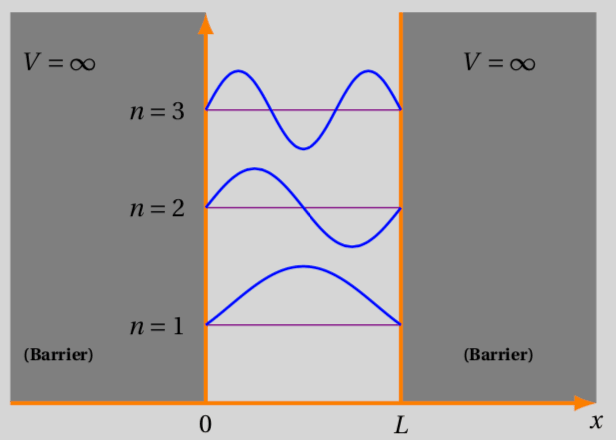
\includegraphics[scale = 0.4]{PIAB.png} \\ \\ 
\textbf{Particle in a Quantum Well}\\ \\ 
\textbf{Finite Quantum Well Derivation} \\ \\
A finite quantum well, also known as a finite square well, is a concept in quantum mechanics where a particle is confined within a "box" with finite potential "walls". The potential function is defined as:
$$
V(x) = \begin{cases}
-V_0, & |x| \leq L \\
0, & |x| > L
\end{cases}
$$
where $V_0$ is the depth of the well, and $L$ is the width of the well.\\
\textbf{Wave Function and Schrödinger Equation}\\ \\
To find the wave function and energy eigenvalues, we need to solve the time-independent Schrödinger equation (TISE):
$$
-\frac{\hbar^2}{2m}\frac{d^2\psi(x)}{dx^2} + V(x)\psi(x) = E\psi(x)
$$
The TISE can be divided into three regions:
1. Region I ($x < -L$): $V(x) = 0$
2. Region II ($-L \leq x \leq L$): $V(x) = -V_0$
3. Region III ($x > L$): $V(x) = 0$
For regions I and III, the TISE becomes:
$$
-\frac{\hbar^2}{2m}\frac{d^2\psi(x)}{dx^2} = E\psi(x)
$$
The general solution for regions I and III is:
$$
\psi_I(x) = Ae^{k_1x} + Be^{-k_1x}, \quad \psi_{III}(x) = Fe^{k_1x} + Ge^{-k_1x}
$$
where $k_1 = \sqrt{\frac{2mE}{\hbar^2}}$.
For region II, the TISE becomes:
$$
-\frac{\hbar^2}{2m}\frac{d^2\psi(x)}{dx^2} - V_0\psi(x) = E\psi(x)
$$
The general solution for region II is:
$$
\psi_{II}(x) = C\cos(k_2x) + D\sin(k_2x)
$$
where $k_2 = \sqrt{\frac{2m(E + V_0)}{\hbar^2}}$. \\ \\
\textbf{Boundary Conditions and Matching Solutions}\\ \\
The wave function and its first derivative must be continuous at the boundaries $x = \pm L$ . Therefore, we have the following boundary conditions:\\
\begin{itemize}
    \item $\psi_I(-L) = \psi_{II}(-L) $
    \item $\psi_{II}(L) = \psi_{III}(L)$
    \item $\psi_I'(-L) = \psi_{II}'(-L)$
    \item $\psi_{II}'(L) = \psi_{III}'(L)$
    \end{itemize}
Applying these boundary conditions and exploiting the symmetry of the problem, we can reduce the number of unknown coefficients and obtain transcendental equations for the allowed energies. For even parity solutions, we have:
$$
\alpha\tan(\alpha) = k_2
$$
For odd parity solutions, we have:
$$
\alpha\cot(\alpha) = -k_2
$$
where $\alpha = k_1L$. 
\newpage
\section{ Lecture 11}

\textbf{Quantum Tunneling} \\ \\
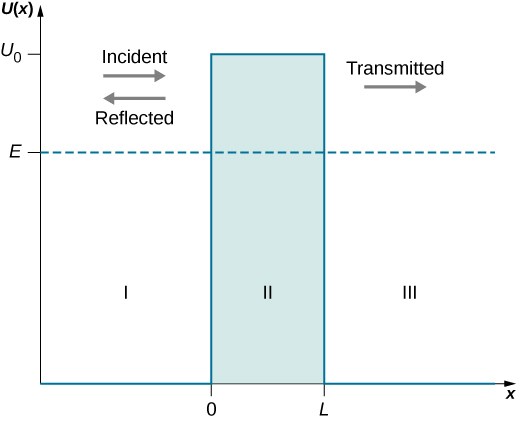
\includegraphics[]{QuantumTunneling.jpg} \\ \\ 
\href{https://spot.colorado.edu/~rehnd/heuristics/pdf/tunnelingSummary.pdf}{\color{blue}Supplementary Material Link} \\
The wave-function solution has the the following form:
$$\psi(x) = \begin{cases}
    Ae^{ikx} + B e^{-ikx}, \ \ x<0 \\
    Ce^{-\kappa x}+De^{\kappa x}, \ \ 0 \leq x \leq a \\
    t(A)Ae^{ikx}, \ \ x>a
\end{cases}
$$
Substituting this solution in the Schrödinger equation, for the first two cases$(x\leq a)$ we get that:
$$ k =  \frac{\sqrt{{2m}(E_x-V_0)}}{\hslash}$$
$$ \kappa = \frac{\sqrt{2m(V_0-E)}}{\hslash} $$

We get that:
$$p(x< \zeroslash,v>0) \varpropto |A|^2$$
$$p(x< \zeroslash,v<0) \varpropto |B|^2$$
$$p(x>a,v>0) \varpropto|t(A)|^2 |A|^2$$
$$|t|^2 = \frac{p(x< \zeroslash,v>0)}{p(x> \zeroslash,v>0)}$$
We will make some assumptions, which will make the discussion easier. Let's assume that D is negligible, the probability that the particle is reflected at the second barrier is considered null. Thus we can assume that $D=0$. Now as a boundary condition we impose the continuity of the wave function:
$$ \begin{cases}  
 \psi(0^+) = \psi(0^-) \implies A+B = C \\
 \psi(a^+) = \psi(a^-) \implies Ce^{-\kappa a} = tAe^{ika} \\
\end{cases}
$$
$$\implies (A+B)e^{-\kappa a} = tAe^{ika} \implies t = \frac{A+B}{A}e^{(-\kappa a+ik a)}$$
$$\implies |t|^2 = \frac{|A+B|^2}{|A|^2} e^{-(\kappa a +ik a)} \cdot e^{-(\kappa a-ika)} = \frac{|A+B|^2}{|A|^2}  e^{-2\kappa a} = \beta e^{-2\kappa a} $$
$$|t|^2 = \beta e^{-2a \frac{\sqrt{2m(V_0-E)}}{\hslash}}$$
This last value is just the tunneling probability. \\
\textbf{Ammonia Molecule} \\ 
$$
\begin{cases}
    m_1 \frac{d^2 x_1}{dt^2} &= F(x_1 - x_2) \\
 m_2 \frac{d^2 x_1}{dt^2} &= - F(x_1 - x_2) \\
\end{cases} \implies \begin{cases}
   \frac{d^2 x_1}{dt^2} &=  \frac{F(x_1 - x_2)}{m_1} \\
   \frac{d^2 x_2}{dt^2} &= -\frac{F(x_1-x_2)}{m_2} \\
\end{cases} $$
$$
\frac{d^2 (x_1 - x_2)}{dt^2} = \frac{F}{m_1} (x_1 - x_2) + \frac{F}{m_2} (x_1 - x_2) \\$$
$$\delta = x_1 - x_2 $$
$$ \frac{d^2 \delta}{dt^2} = \biggl(\frac{1}{m_1} + \frac{1}{m_2} \biggl) F(\delta) $$
$$m_R \frac{d^2 \delta}{dt^2} = F(\delta).
$$
We define $m_r = \frac{m_1m_2}{m_1+m_2}$ the reduced mass.



\section{Lecture 12}
$$\hat{H} = \frac{1}{2} \Bigl[ \frac{\hat{p}_x}{m} + kx^2 \Bigl] = \frac{1}{2} \Biggl[ \frac{-\hslash^2}{m} \frac{\partial^2}{\partial x^2}+ kx^2 \Biggl] $$
Let's assume that:
$$ \psi = Ae^{-\frac{x^2}{\sigma^2}}$$
$$\hat{H}\psi(x) = E\psi(x)$$
We get:
$$\frac{1}{2} \Biggl[ \frac{-\hslash^2}{m} \Biggl( Ae^{-\frac{x^2}{\sigma^2}}\biggl( \frac{2x}{\sigma^2}\biggl)^2 - \frac{2}{\sigma^2} Ae^{\frac{-x^2}{\sigma^2}} \Biggl) + kx^2Ae^{-\frac{x^2}{\sigma^2}}\Biggl] = EAe^{-\frac{x^2}{\sigma^2}}$$
The term $\psi = Ae^{-\frac{x^2}{\sigma^2}} $ can be simplified, obtaining a constant on the right term.
$$\frac{1}{2} \Biggl[ \frac{-\hslash^2}{m} \Biggl(\biggl( \frac{2x}{\sigma^2}\biggl)^2 - \frac{2}{\sigma^2} \Biggl) + kx^2\Biggl] = E$$
By imposing  the following two conditions that the coefficients of the $x^2$ terms are zero and $x=0 $, so the the equation always hold $\forall x$, we get:
\begin{enumerate}
    \item $  x = 0 \implies \ \frac{\hslash^2 }{\sigma^2 m} = E $
    \item Sum of the coefficients of $x^2$ equal to zero, $ \implies \ \frac{-\hslash^2}{m}\Biggl(\frac{2}{\sigma^2}\Biggl)^2+ kx^2 = 0 \implies \ \sigma^2 =  \frac{2 \hslash}{\sqrt{mk}}$
\end{enumerate}
By "substituting" $2.$ into $1.$, we obtain:
$$E = \frac{1}{2}\hslash\sqrt{\frac{k}{m}} = \frac{1}{2}\hslash \omega$$

\begin{gather*}
    \hat{H} = \frac{1}{2}\Biggl[ \frac{-\hslash^2}{m}\frac{d}{dx^2}+kx^2 \Biggl] =\frac{1}{2}\Biggl[ \frac{-\hslash^2}{m}\frac{d}{dx^2}+m\omega^2x^2 \Biggl] = \frac{1}{2} \Biggl[ \frac{\hat{p}_x^2}{m} + m\omega^2 x^2 \Biggl] = \\ = \frac{1}{2} \Biggl[ \hat{\pi}^2 + \omega^2 q^2 \Biggl] = \frac{1}{2}(-i \hat{\pi}+\omega q)(i \hat{\pi}+\omega q).
\end{gather*}
$$\pi = \frac{\hat{p}_x}{\sqrt{m}},\ q = \sqrt{m}x$$


$$\hat{a}^{\dag} \triangleq \bigl( -i\hat{\pi} + \omega q \bigl) \frac{1}{\sqrt{2\hslash\omega}} = \frac{1}{\sqrt{2}} \biggl( \sqrt{\frac{m\omega}{\hslash}}\hat{x}+ i \frac{1}{\sqrt{m\hslash\omega}} \hat{p} \biggl) = \frac{1}{\sqrt{2}} \biggl( \sqrt{\frac{m\omega}{\hslash}}x+  \frac{\hslash}{\sqrt{m\hslash\omega}}  \frac{\partial }{\partial x}\biggl)  $$
    
$$\hat{a} \triangleq \bigl( i\hat{\pi} + \omega q \bigl) \frac{1}{\sqrt{2\hslash\omega}} =  \frac{1}{\sqrt{2}} \biggl( \sqrt{\frac{m\omega}{\hslash}}\hat{x}- i \frac{1}{\sqrt{m\hslash\omega}} \hat{p} \biggl) = \frac{1}{\sqrt{2}} \biggl( \sqrt{\frac{m\omega}{\hslash}}x-  \frac{\hslash}{\sqrt{m\hslash\omega}}  \frac{\partial }{\partial x}\biggl)$$

$$\hat{\pi} = \frac{\hat{p}_x}{\sqrt{m}} = - \frac{i \hslash}{\sqrt{m}} \frac{d}{dx} $$

$$ \hat{H} = \frac{1}{2} \biggl[ \hat{\pi}^2 + \omega^2 q^2 \biggl]$$

\begin{align*}
\hat{a}^{\dag} \cdot \hat{a} \psi = \frac{\hat{a}^{\dag} (i\hat{\pi} + \omega q)}{\sqrt{2\hslash \omega}} \psi = \frac{\hat{a}^{\dag}(i\hat{\pi}\psi+\omega q \psi)}{\sqrt{2\hslash \omega}} = \frac{\hat{a}^{\dag}}{\sqrt{2\hslash\omega}} \Biggl( \frac{\hslash}{\sqrt{m}} \frac{d\psi}{dx} + \omega q \psi \Biggl) = \\ = \frac{1}{2\hslash \omega} \Biggl[ \frac{-\hslash}{\sqrt{m}} \frac{d}{dx} \Biggl( \frac{\hslash}{\sqrt{m}} \frac{d\psi}{dx} + \omega q \psi \Biggl) + \omega q \frac{\hslash}{\sqrt{m}} \frac{d\psi}{dx} + \omega^2q^2\psi\Biggl] = \frac{1}{\hslash \omega} \hat{H} -\frac{1}{2}\psi
\end{align*}

$$\hat{a}^{\dag} = \frac{1}{\sqrt{2\hslash\omega}} ( -i\hat{\pi}+\omega q) = \frac{1}{\sqrt{2\hslash\omega}} \Bigl( -\hslash\frac{d}{dx}+ m\omega x \Bigl)$$

$$\hat{a} = \frac{1}{\sqrt{2\hslash\omega}} (i\hat{\pi}+\omega q) = \frac{1}{\sqrt{2\hslash\omega}} \Bigl(\hslash\frac{d}{dx}+ m\omega x \Bigl)$$

$$\hat{H} = \frac{1}{2} \hslash \omega \bigl[\hat{a}^{\dag}\hat{a} +\hat{a}\hat{a}^{\dag} \bigl] $$
$$\hat{H} = \hslash \omega \bigl[ \hat{a}^{\dag} \hat{a} + \frac{1}{2}\bigl] $$
$$\hat{H} = \hslash \omega \bigl[\hat{a} \hat{a}^{\dag} - \frac{1}{2}\bigl] $$
Note that $\hat{a}$ and $\hat{a}^{\dag}$ are not Hermitian Operator. One is the adjoint operator of the other. However their product is Hermitian.

$$ 0 = \hslash \omega \Bigl( \hat{a}^{\dag} \hat{a} + \frac{1}{2} - \hat{a}^{\dag}\hat{a} + \frac{1}{2} \Bigl) $$
$$[\hat{a},\hat{a}^{\dag}] = \hat{a}\hat{a}^{\dag} - \hat{a}^{\dag}\hat{a} = 1$$

$$\hat{H}\hat{a}^{\dag} = \hslash \omega \biggl( \hat{a}^{\dag}\hat{a}\hat{a}^{\dag}+ \frac{1}{2}\hat{a}^{\dag} \biggl) $$
$$\hat{a}^{\dag} \hat{H} =  \hslash \omega \biggl( \hat{a}^{\dag}\hat{a}^{\dag}\hat{a}+ \frac{1}{2}\hat{a}^{\dag} \biggl)$$
When we subtract these two equations:
$$ [\hat{H}, \hat{a}^{\dag}] = \hslash\omega\hat{a}^{\dag}[\hat{a}^{\dag},\hat{a}] = \hslash\omega\hat{a}^{\dag} $$
Equivalently:
$$[\hat{H}, \hat{a}] = -\hslash\omega\hat{a}$$
Let's talk about different energy levels:
$$\hat{H}\ket{n} = E_n \ket{n}$$
$$ \hat{H}\hat{a}^{ \dag} = \hslash \omega \hat{a}^{\dag} + \hat{a}^{\dag}\hat{H}$$
$$\hat{H}\hat{a}^{\dag} \ket{n} = \hslash \omega \hat{a}^{\dag} \ket{n} + \hat{a}^{\dag}\hat{H}\ket{n} = \hslash\omega\hat{a}^{\dag}\ket{n} + E_n \hat{a}^{\dag}\ket{n}$$
$$\hat{H}(\hat{a}^{\dag}\ket{n}) = (\hslash\omega+E_n)(\hat{a}^{\dag}\ket{n})$$
$$\hat{H}\ket{n+1} = (\hslash\omega + E_n ) \ket{n+1}$$
\begin{equation*}
\begin{rcases}
  E_{n+1} = \hslash \omega + E_n \\
  E_0= \frac{1}{2} \hslash \omega \\
\end{rcases}
\implies E_n = \hslash \omega \biggl( n + \frac{1}{2} \biggl)
\end{equation*} 
Similarly, for $\hat{a}$, you can demonstrate that:
$$\hat{H}\bigl( \hat{a}\ket{n} \bigl) = (E_n -\hslash \omega ) (\hat{a}\ket{n}) = (E_n -\hslash \omega) \ket{n-1} $$
This notation is called occupancy number representation.\\
Now, we can express the position and momentum operators in terms of the raising and lowering operators:

$$
\hat{x} = \sqrt{\frac{\hbar}{2m\omega}}(\hat{a} + \hat{a}^\dagger)
$$

$$
\hat{p} = i\sqrt{\frac{m\hbar\omega}{2}}(\hat{a}^\dagger - \hat{a})
$$



\section{Lecture 13}
Assume that we are working with unitary kets, thus $\bra{n}\ket{n} = 1$.
$$\hat{H}\hat{a}^{\dag} \ket{n} = (E_n + \hslash \omega ) \hat{a}^{\dag}\ket{n} = (E_n + \hslash \omega ) c\ket{n+1} $$
$$\hat{H}\hat{a} \ket{n} = (E_n -\hslash \omega) \hat{a}\ket{n} = (E_n -\hslash \omega) c' \ket{n-1} $$
\begin{flalign*}
   c^2 = c^2 \bra{n+1}\ket{n+1} =  \biggl(\bra{n} \bigl( \hat{a}^\dag \bigl) ^\dag \biggl) \biggl(\hat{a}^{\dag}\ket{n} \biggl) = \bra{n}\hat{a}\hat{a}^{\dag}\ket{n} = \star
\end{flalign*}
Now, remembering that:
$$\hat{H} = \hslash \omega \biggl(\hat{a}\hat{a}^{\dag}-\frac{1}{2} \biggl) \implies  \frac{1}{\hslash \omega}\hat{H} + \frac{1}{2} = \hat{a}\hat{a}^{\dag}$$
 \begin{equation*}
     \star = \bra{n}\frac{1}{\hslash \omega} \hat{H}\ket{n}+\frac{1}{2} \bra{n}\ket{n} = \frac{1}{\hslash\omega}\bra{n}\hat{H}\ket{n}+\frac{1}{2} = \frac{1}{\hslash\omega}E_n + \frac{1}{2} = \frac{1}{\hslash\omega}\hslash\omega\biggl( n+\frac{1}{2} \biggl) + \frac{1}{2} = n+1.
 \end{equation*}
As a convention for $c$ we choose a positive number. There is no physical reason why it cannot be the opposite.
$$\implies c = +\sqrt{n+1}$$
Reasoning in the same way, remembering that $ \hat{H} = \hslash \omega \bigg(\hat{a}^\dag + \frac{1}{2} \biggl)$:
\begin{gather*}
    c'^2= {c'}^2 \bra{n}\ket{n} = \bigl( \bra{n}\hat{a}^{\dag}\bigl) \bigl( \hat{a}\ket{n} \bigl) = \bra{n}\frac{\hat{H}}{\hslash \omega}-\frac{1}{2}\ket{n} = n + \frac{1}{2}-\frac{1}{2} =n. 
\end{gather*}
$$ V = \frac{1}{2}kx^2$$
$$ \hat{a}^{\dag} \triangleq \frac{1}{\sqrt{2\hslash\omega}}(-i\hat{\pi}+\omega q) \triangleq  \frac{1}{\sqrt{2\hslash\omega}}\bigl( \frac{i}{\sqrt{m}}\hat{p}_x + \sqrt{m}\omega x \bigl) = \frac{1}{\sqrt{2\hslash m \omega}}\bigl( i \hat{p}_x + m \omega x \bigl) $$
$$\hat{a} = \frac{1}{\sqrt{2\hslash m \omega}}\bigl(- i \hat{p}_x + m \omega x \bigl) $$
$$\implies \hat{a}+\hat{a}^{\dag} = \frac{2}{\sqrt{2\hslash m \omega}}(m\omega x) = \sqrt{\frac{2m\omega}{\hslash}}x  \implies x = \sqrt{\frac{\hslash}{2m\omega}} (\hat{a}^{\dag}+\hat{a})$$
$$ \langle V \rangle = \bra{n}V \ket{n} = \bra{n}\frac{1}{2}kx^2 \ket{n} = \frac{1}{2} k \frac{\hslash}{2m\omega} \bra{n}(\hat{a}^{\dag} + \hat{a})(\hat{a}^{\dag}+\hat{a})\ket{n} = \frac{1}{2}k \frac{\hslash}{2m\omega} \bra{n}\hat{a}^{\dag}\hat{a}^{\dag}+ \hat{a}^{\dag}\hat{a}+\hat{a}\hat{a}^{\dag}
+\hat{a}\hat{a}\ket{n} = \star $$ 
The first and last term between the bra and the ket generate $\ket{n+2}$ and $\ket{n-2}$, which are orthogonal to $\ket{n}$, thus:
$$\star = \frac{1}{2}k \frac{\hslash}{2m\omega} \bra{n}\hat{a}^{\dag}\hat{a}+\hat{a}\hat{a}^{\dag} \ket{n} = \star \star$$
Remembering that:
$$\hat{H} = \frac{\hslash\omega}{2}(\hat{a}^{\dag}\hat{a}+\hat{a}\hat{a}^{\dag}) \implies \hat{a}^{\dag}\hat{a}+\hat{a}\hat{a}^{\dag} = \frac{2\hat{H}}{\hslash\omega} $$
$$ \star \star = \frac{1}{2} k \bra{n}\frac{2\hat{H}}{\hslash\omega}\ket{n}\frac{\hslash}{2m\omega}=\frac{k}{2m\omega^2}\bra{n}\hat{H}\ket{n}=\frac{m\omega^2}{2m\omega^2}\bra{n}\hat{H}\ket{n}=\frac{1}{2}\langle E_n \rangle = \frac{1}{2}E_n$$
$$\langle K \rangle = E_{TOT} -\langle V \rangle = \frac{1}{2} E_n$$
Equipartition of energy theorem for harmonic Oscillator.

$$ \hat{a}^{\dag}(\hat{a} \ket{n}) = \hat{a}^{\dag}\sqrt{n}\ket{n-1} =\sqrt{n}\hat{a}^\dag \ket{n-1}= \sqrt{n}\sqrt{n}\ket{n} = n \ket{n}$$
Thus we call $\hat{a}^{\dag}\hat{a} = \hat{n}$, the occupation  number operator.\\  \\ 
\textbf{Harmonic Oscillator CO2 }\\ \\
We will describe at first the system from a classical point of view.
Notation:$ x_c,x_1,x_2 $ indicate the position of the carbon atom, and the $ 1^{st}$and $2^{nd} $ oxygen atom respectively.
$$F_x = F(x_c-x_1) = F_x(\delta)$$
$$F_x  \cong F_x(\delta_0)+ \frac{dF_x(\delta_0)}{d\delta}(\delta-\delta_0) = 0 -k (\delta-\delta_0)$$
Here $\delta_0$ identifies the equilibrium distance, thus the force $F(\delta_0) = 0.$
We can write:
$$m_o \frac{d^2x_1}{dt^2} = -k(x_1-x_c)$$
$$m_o \frac{d^2x_2}{dt^2} = -k(x_2-x_c)$$
$$m_c \frac{d^2x_c}{dt^2} = -k(x_c-x_1)-k(x_c-x_2)$$
$$\implies\frac{d^2}{dt^2} (m_o x_1+m_0x_2+m_c x_c) = \frac{dx_{CM}}{dx^2} = 0$$
From the first two equations:
$$m_o \frac{d^2x_1}{dt^2}-m_o \frac{d^2x_2}{dt^2} = -k(x_1-x_c)+k(x_2-x_c)$$
$$\implies m_0 \frac{d^2}{dt^2}(x_1-x_2) = -k(x_1-x_2)$$
$$ m_o \frac{d^2}{dt^2}A_{oo} = -kA_{oo}$$
$$ \frac{d^2}{dt^2}A_{oo} +\frac{k}{m_o}A_{00}=0 \implies \omega_\gamma = \sqrt{\frac{k}{m_0}}$$
This is the first oscillating mode. There is another one. From the $3^{rd}$ equation we get:
$$m_c \frac{d^2x_c}{dt^2} = -k(2x_c-x_1-x_2)$$
$$\implies \frac{d^2x_1}{dt^2}+\frac{d^2x_2}{dt^2}-2\frac{d^2x_c}{dt^2} = -\frac{k}{m_o} (x_1-x_c)-\frac{k}{m_o} (x_2-x_c)+2\frac{k}{m_c}(2x_c-x_1-x_2)$$
$$\frac{d^2}{dt^2}(x_1+x_2-2x_c) = -\frac{k}{m_o}(x_1+x_2-2x_c)+\frac{2k}{m_c}(2x_c-x_1-x_2)$$
$$\frac{d^2}{dt^2}(x_1+x_2-2x_c) = -\biggl(\frac{k}{m_o}+\frac{2k}{m_c}\biggl)(x_1+x_2-2x_c)$$
$$\frac{d^2}{dt^2}(x_1+x_2-2x_c) + \biggl(\frac{k}{m_o}+\frac{2k}{m_c}\biggl)\biggl(x_1+x_2-2x_c\biggl) = 0 \implies\omega_u = \sqrt{\frac{k(m_c+2m_o)}{m_om_c}}$$
\section{Lecture 14} 
From now on we will consider time evolution, so we will introduce the time variable. 
Let's introduce the time translation operator, with the following properties:
$$\hat{t}_{\tau} \ket{u(t)} = \ket{u(t+\tau)}$$
$$\hat{t}_{\tau}(\ket{u(t)}+\ket{v(t)}) = \ket{u(t+\tau)}+ \ket{v(t+\tau)}$$
$$\hat{t}_{\tau}(\alpha\ket{u(t)}) = \alpha \ket{u(t+\tau)}$$
$$\hat{t}_{\tau_1} \hat{t}_{\tau_2} \ket{u(t)} = \hat{t}_{\tau_1}\ket{u(t+\tau_2)}=\ket{u(t+\tau_1+\tau_2)}= \hat{t}_{\tau_2}\hat{t}_{\tau_1}\ket{u(t)}$$
$$\hat{t}_{\tau_1}\ket{\psi(t)} = \beta_{\tau_1}\ket{\psi(t)}= \ket{\psi(t+\tau_1)}$$
$$\hat{t}_{\tau_2}\ket{\psi(t)} = \beta_{\tau_2}\ket{\psi(t)}= \ket{\psi(t+\tau_2)}$$
$$\beta_{\tau_1}\beta_{\tau_2}\ket{\psi(t)}=\hat{t}_{\tau_1} \hat{t}_{\tau_2} \ket{\psi(t)} = \hat{t}_{\tau_1+\tau_2} \ket{\psi(t)} = \beta_{\tau_1+\tau_2}\ket{\psi(t)}$$
$$\implies \beta_{\tau_1+\tau_2} = \beta(\tau_1+\tau_2) = \beta_{\tau_1}\beta_{\tau_2} = \beta(\tau_1)\beta(\tau_2) \implies \beta(t) = e^{-i\omega t}, \omega \in \mathbb{R}$$
The condition of $\omega$ belonging to the reals, is due to the fact that it must hold the following: $|\beta(t)|^2 = 1$.
$$\ket{\psi(t)} = \hat{t}_\tau \ket{\psi(t=0)} = \beta(t)\ket{\psi(t=0)}=e^{-i\omega t} \ket{\psi(t=0)}$$
Let's remember that, the conservation of energy imposes:
$$\hat{H}\ket{\psi(t=0)} = E \ket{\psi(t=0)} \implies \hat{H}\hat{t}_{\tau_2}\ket{\psi(t=0)} = E \hat{t}_{\tau_2} \ket{\psi(t=0)}$$
$$\hat{H} \ket{\psi(t=0)} = E \ket{\psi(t=0)} $$
$$\hat{H} \hat{t}_{\tau_2} \ket{\psi(t=0)} = E \hat{t}_{\tau_2} \ket{\psi(t=0)}$$
The second equation can be rewritten as:
$$\hat{t}_{\tau_2}^{-1} \hat{H} \hat{t}_{\tau_2} \ket{\psi(t=0)} = E \ket{\psi(t=0)}
$$
Comparing the first and the rewritten second equation, we can see that:
$$\hat{t}_{\tau_2}^{-1} \hat{H} \hat{t}_{\tau_2} = \hat{H}$$
Multiplying both sides by $\hat{t}_{\tau_2}$, we get:
$$
\hat{H} \hat{t}_{\tau_2} = \hat{t}_{\tau_2} \hat{H}
$$
So we have proved that the time translation operator and the Hamiltonian operator commute, thus they share the same set of eigenfunctions. So there is a one-to-one correspondence of the eigenfunctions, thus $\omega  = f(E)$ must be a function of the energy.\\
Let's assume to have two non interacting particles, so there is no energy associated with the interaction. The total energy is the sum of the energies of the single particles.
$$\ket{\psi_{TOT}} = \ket{\psi_1(t)}\ket{\psi_2(t)} = \ket{\psi_1(t=0)}e^{-i\omega_1t}\ket{\psi_2(t=0)}e^{-i\omega_2 t} = \ket{\psi_1(t=0)}\ket{\psi_2(t=0)}e^{-i(\omega_1+\omega_2)t}$$
$$\implies f(E_1+E_2) = \omega_1 + \omega_2 = f(E_1)+ f(E_2) \implies \omega \varpropto E$$
\textbf{Photons} \\
Photons have no mass, so $E = \sqrt{c^2p^2+m^2c^4} = \sqrt{c^2p^2} = cp$
$$e^{i(kx-\omega t)}, \ c = \frac{\omega}{k}, \ p = \hslash k \implies p =  \frac{\hslash\omega}{c}, E = \hslash \omega$$
$$\hat{H}\ket{\psi(t=0)} = E \ket{\psi(t=0)}  \implies \ket{\psi(t)} = e^{-i\frac{E}{\hslash}t} \ket{\psi(t=0)}$$
Remember that we are assuming that $\psi$ is an eigenfunction of the Hamiltonian operator.
For a generic quantum state, the following holds true:
$$\ket{u(t)} = \sum_j \alpha_j e^{-i\frac{E_j}{\hslash}t} \ket{\psi_j(t=0)}$$
$$\ket{u(t=0)} = \sum_j \alpha_j \ket{\psi_j(t=0)}$$
$$H\ket{\psi_j(t=0)} = E_j \ket{\psi_j(t=0)}$$ \\ 
$$\hat{H} = \begin{bmatrix}
    0 & -\frac{\Delta E}{2} \\
    -\frac{\Delta E}{2} & 0 \\
\end{bmatrix} \begin{bmatrix}
    \alpha_1  \\
      \alpha_2 \\
\end{bmatrix} = E \begin{bmatrix}
    \alpha_1  \\
      \alpha_2 \\
\end{bmatrix} \implies E = \pm \frac{\Delta E}{2}$$ 
$$\frac{1}{\sqrt{2}}  \begin{bmatrix}
    1 \\
    1 \\
\end{bmatrix} = \ket{g}, \frac{1}{\sqrt{2}} \begin{bmatrix}
    1 \\
    -1 \\
\end{bmatrix} = \ket{u}$$

$$\ket{u(t=0)} = \alpha \ket{g} + \beta \ket{u}$$
$$|\alpha|^2+|\beta|^2 = 1$$
$$\ket{u(t)}= \alpha e^{i \frac{\Delta E}{2 \hslash}t} \ket{g}+ \beta e^{-i \frac{\Delta E}{2 \hslash}t} \ket{u}$$
$$\langle x \rangle  = \bra{u(t)} \hat{x} \ket{u(t)} =\ket{u(t)}^T \begin{bmatrix}
    x_0 & 0 \\
    0 & -x_0 \\
\end{bmatrix} \ket{u(t)} =2 x_0 \alpha \beta \biggl( e^{i \frac{\Delta E t}{2 \hslash}} \biggl) =2 x_0 \alpha \beta cos\biggl(\frac{\Delta E}{\hslash}t\biggl)$$
If we assume that $\alpha, \beta \in \mathbb{R} \implies a = \alpha^*, \beta = \beta^*$. 

\section{Lecture 15}
Let $E_j' = E_j + E_0$.
$$\ket{u(t)} = \sum_j \alpha_j e^{-i\frac{E_j}{\hslash}t} \ket{\psi_j}$$
$$\ket{u(t)} = \sum_j \alpha_j e^{-i\frac{E_j'-E_0}{\hslash}t} \ket{\psi_j} $$
$$\ket{u(t)} = \Biggl( \sum_j \alpha_j e^{-i\frac{E_j'}{\hslash}t} \ket{\psi_J} \Biggl) e^{i \frac{E_0}{\hslash}t} = \ket{u'(t)}  e^{i \frac{E_0}{\hslash}t} $$
Obviously $\ket{u(t)}$ and $\ket{u'(t)}$ represent the same quantum state, so $E_0$ can be chosen arbitrarily. \\ \\
\textbf{Dynamics of a free particle}
$$\hat{H} = \frac{-\hslash^2}{2m} \nabla^2$$
In one dimension:
$$\hat{H}\psi{x} = E \psi(x) \implies \frac{-\hslash^2}{2m} \frac{d^2 \psi(x)}{dx} - E \psi(x) = 0$$
The solution is $\psi(x) = e^{ikx}$, and if we introduce time dependence we get: $ \psi(x,t) = e^{i(kx-\omega t)}$ with: $ \hslash k = p, \hslash \omega = E.$

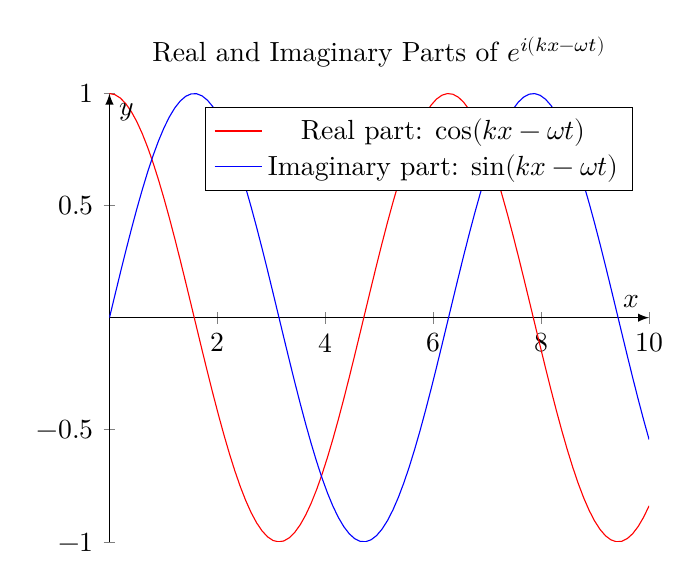
\begin{tikzpicture}
\begin{axis}[
    xlabel={$x$},
    ylabel={$y$},
    legend pos=north east,
    title={Real and Imaginary Parts of $e^{i(kx-\omega t)}$},
    axis lines=center,
    axis line style={-latex}]
\addplot[domain=0:10, samples=100, red] {cos(deg(x))};
\addlegendentry{Real part: $\cos(kx-\omega t)$}
\addplot[domain=0:10, samples=100, blue] {sin(deg(x))};
\addlegendentry{Imaginary part: $\sin(kx-\omega t)$}
\end{axis}
\end{tikzpicture} \\
Let's apply a change of coordinate, with the observer moving at the same speed of the wave:
$$x'=x-vt$$
This value: $ e^{i(kx'+kvt-\omega t)}$ is constant when $kv = \omega \implies v = \frac{\omega}{k}$.
$$\hslash k = p$$
$$\hslash \omega = E= \frac{p^2}{2m} = \frac{pv}{2} \implies v = \frac{2E}{p} = 2\frac{\hslash \omega}{\hslash k} = \frac{2\omega}{k}\neq \frac{\omega}{k}$$
So there is a paradox, because we obtain two different velocities.
Let's switch to momentum representation, and remembering that $\omega = \frac{p^2}{2m\hslash}$.
$$\Psi(p,t) = \Psi(p) e^{-i\omega (p) t}$$
$$\langle \hat{X} \rangle = \bra{\Psi(p,t)} \hat{X} \ket{\Psi (p,t)}$$
$$\hat{X}\Psi(p,t) = i\hslash\frac{d}{dp} \biggl[ \Psi(p) e^{-i\omega(p)t} \biggl] = i \hslash \biggl[ e^{-i\omega (p) t} \frac{d \Psi(p)}{dp} + \Psi(p) \biggl(-it \frac{d\omega(p)}{dp} \biggl)  e^{-i \omega(p)t} \biggl] $$

\begin{flalign*}
& \bra{\Psi(p,t)} \hat{X} \ket{\Psi(p,t)} = i \hslash e^{i \omega(p)t} \bra{\Psi(p)} \ket{ \frac{d\Psi(p)}{dp} + \Psi(p) \biggl( -it \frac{d\omega(p)}{dp} \biggl) } e^{-i \omega(p)t} = &\\
& i \hslash \bra{\Psi(p)} \ket{ \frac{d\Psi(p)}{dp}} + \hslash t \bra{\Psi(p)}\frac{d\omega(p)}{dp}\ket{\Psi(p)}= \bra{\Psi(p)} i\hslash \frac{d}{dp} \ket{\Psi(p)} + \hslash t   \bra{\Psi(p)} \frac{p}{m\hslash} \ket{\Psi(p)} = &\\ 
& \langle  \hat{X} \rangle_{t=0} + \frac{t}{m}  \bra{\Psi(p)} p \ket{\Psi(p)} = \langle \hat{X} \rangle_{t=0} + \frac{t}{m} \langle \hat{p} \rangle = \langle x(t=0) \rangle + \langle \hat{v} \rangle  t 
\end{flalign*} \\ \\
We define $\hat{v} = \hslash \frac{d\omega(p)}{dp} = \frac{d\omega}{dk}$ = "group \ velocity" $\neq \frac{\omega}{k} =$ "phase velocity"  \\ \\
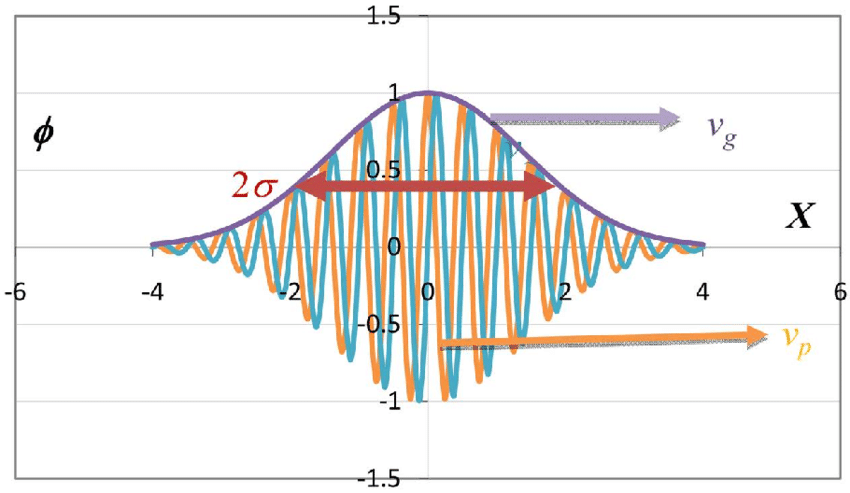
\includegraphics[scale = 0.5]{phase-group-velocity.png} \\ \\ 
In free space, a particle become more dispersed.
$$\Psi(p,t) = e^{-i\omega(p)t}$$
$$\ket{u(t)} = \sum_j \alpha_j e^{-i\frac{E_j}{\hslash}t} \ket{\psi(j)}$$
$$\hat{H}\ket{\psi_j} = E_j \ket{\psi_j}$$
$$u(t+\Delta t) = \sum_j \alpha_j e^{-i\frac{E_j}{\hslash}(t+\Delta t)}\ket{\psi_j}$$
$$\implies \frac{\ket{u(t+\Delta t)} - \ket{u(t)}}{\Delta t} = \sum_j \alpha_j e^{\frac{-iE_j t}{\hslash}}  \frac{e^{\frac{-iE_j\Delta t}{\hslash}}-1}{\Delta t} \ket{\psi_j} $$
For $ t \longrightarrow 0 $:
$$\frac{ \partial \ket{u(t)}}{\partial t} = -\frac{i}{\hslash} \sum_j \alpha_j e^{\frac{-iE_jt}{\hslash}} E_j \ket{\psi_j}  \implies \frac{\partial\ket{u(t)}}{\partial t} = -\frac{i}{\hslash}\hat{H}\sum_j \alpha_j e^{\frac{-iE_j t}{\hslash}}\ket{\psi_j} $$
We finally get the time dependent Schrodinger Equation:
$$\frac{ \partial \ket{u(t)}}{\partial t} = \frac{-i}{\hslash}\hat{H}\ket{u(t)} \implies \hat{H} \ket{u(t)} = \hslash i \frac{\partial \ket{u(t)}}{\partial t} $$
If we can factor: $ \ket{u(t)} = u(x,t) = \psi(x) T(t)$, and $\hat{H}$ doesn't depend on time, so $\hat{H}$ only acts on $\psi$  we get:
$$\hat{H}\psi(x) T(t) = i \hslash \frac{\partial}{\partial t} \bigl[ u(x,t) \bigl] \implies T(t) \hat{H}\psi(x) = i \hslash \psi(x) \frac{\partial}{\partial t} T(t) \implies \hat{H} = i \hslash \frac{1}{T(t)} \frac{d T(t)}{dt} = E$$
The left term doesn't depend on time, the right one doesn't depend on position, so they must be constant, so $E=c$.
We obtain again the time independent Shrodinger Equation.
$$\hat{H}\psi(x) = E \psi(x)$$
$$i \hslash \frac{dT(t)}{dt} = E T(t)$$
$$T(t) \varpropto e^{-\frac{E}{\hslash}t}$$

\section{Lecture 16}
\textbf{Ehrenfest Theorem}

$$\frac{d}{dt} \langle \hat{O} \rangle = \frac{d}{dt} \bra{u} \hat{O} \ket{u} = \bra{\frac{\partial u}{\partial t}} \hat{O} \ket{u} + \bra{u} \frac{\partial \hat{O}}{\partial t} \ket{u} + \bra{u} \hat{O} \ket{\frac{\partial }{\partial t}u}$$
From the time dependent Shrodinger equation we have that: $\frac{\partial u}{\partial t} = \frac{1}{i\hslash} \hat{H}\ket{u} $
Thus, substituting and using the complex conjugate when switching from a ket to a bra:
$$\frac{d}{dt} \langle \hat{O} \rangle = \bra{-\frac{1}{i\hslash} \hat{H} u} \hat{O} \ket{u} + \biggl\langle \frac{\partial \hat{O}}{\partial t} \biggl\rangle + \bra{u} \hat{O} \ket{\frac{1}{i\hslash} \hat{H} u}  = -\frac{1}{i\hslash}  \bra{\hat{H} u} \hat{O} \ket{u} + \biggl\langle \frac{\partial \hat{O}}{\partial t} \biggl\rangle + \frac{1}{i\hslash} \bra{u} \hat{O}  \ket{\hat{H} u} 
$$
We can now exploit the Hermeticity of the operator, and we get:
$$\frac{d}{dt} \langle \hat{O} \rangle = -\frac{1}{i\hslash}  \bra{ u} \hat{H}\hat{O} \ket{u} + \biggl\langle \frac{\partial \hat{O}}{\partial t} \biggl\rangle + \frac{1}{i\hslash} \bra{u} \hat{O} \hat{H} \ket{u} = \frac{1}{i\hslash} \bra{u} \hat{O}\hat{H}- \hat{H}\hat{O} \ket{u} + \biggl\langle \frac{\partial \hat{O}}{\partial t} \biggl\rangle $$
$$ \implies \frac{d}{dt} \langle \hat{O} \rangle = \frac{1}{i\hslash}\bra{u}[\hat{O}, \hat{H}] \ket{u} +  \biggl\langle \frac{\partial \hat{O}}{\partial t} \biggl\rangle $$
For the position operator the last term is null, since position operator doesn't depend on time:
$$\frac{dx}{dt} =  \frac{1}{i\hslash}\bra{u}[x, \hat{H}] \ket{u}$$
Let's remember that:
$[x,\hat{H}] = [x, \hat{K}+ \hat{V}] = [x,\hat{K}]+ [x, \hat{V}] = [x,\hat{K}] $, since  the potential operator depends only on the position of the particle. As both terms in the commutator involve multiplication by the same function of position, they are equal, and the commutator is zero.

\begin{flalign*}
\bigl[x,\hat{K}\bigl] \psi(x) = \frac{-\hslash^2}{2m} \biggl[ x \frac{d^2 \psi(x)}{dx^2} - \frac{d^2}{dx^2} x \psi(x) \biggl] = \frac{-\hslash^2}{2m} \Biggl[ x \frac{d^2 \psi(x)}{dx^2} -  \frac{d}{dx} \biggl( \psi(x) + x \frac{d}{dx} \psi(x) \biggl) \Biggl] = \\   \frac{-\hslash^2}{2m} \biggl[ x \frac{d^2 \psi(x)}{dx^2} -  \frac{d\psi(x)}{dx}  -  \frac{d\psi(x)}{dx} - x \frac{d^2 \psi(x)}{dx^2} \biggl] = \frac{\hslash^2}{m} \frac{d\psi(x)}{dx}= i \frac{\hslash}{m} \Bigl[ -i\hslash \frac{d}{dx} \Bigl] \psi(x) = \frac{i \hslash}{m} \hat{p}_x \psi(x)
\end{flalign*}

$$\frac{d}{dt} \langle \hat{x} \rangle = \frac{1}{i \hslash} \bra{u} [x, \hat{H} ] \ket{u}  = \frac{1}{i \hslash} \bra{u} \frac{i \hslash}{m} \hat{p}_x \ket{u} = \bra{u}\frac{\hat{p}_x}{m} \ket{u}  = \bra{u} \hat{v}_x \ket{u} = \langle v_x \rangle  $$

\begin{gather*}
 [ \hat{p}_x, V ] \psi(x) = \hat{p}_x V(x) \psi(x) - V(x)\hat{p}_x \psi(x) = -i \hslash  \biggl\{ \frac{d}{dx} [V(x)\psi(x)] - V(x) \frac{d\psi(x)}{dx} \biggl\} = \\ = -i \hslash  \biggl\{ \psi(x) \frac{dV(x)}{dx}+ V(x) \frac{d\psi(x)}{dx} - V(x) \frac{d\psi(x)}{dx} \biggl\} = - i \hslash \psi(x) \frac{dV(x)}{dx}   = i \hslash F_x \psi(x)  \\ \implies [\hat{p}_x,\hat{H}] = i \hslash F_x
\end{gather*}
$$[\hat{p}_x,\hat{H}] = [\hat{p}_x, \hat{K} + \hat{V}] = [ \hat{p}_x, \hat{K} ] + [ \hat{p}_x, \hat{V} ] = \biggl[\hat{p}_x, \frac{\hat{p}_x^2}{2m} \biggl] +   [ \hat{p}_x, \hat{V} ] = 0 +  [ \hat{p}_x, \hat{V} ]  $$
$$\frac{d\langle \hat{p}_x \rangle}{dt} = \frac{1}{i\hslash} \bra{u} [\hat{p}_x,\hat{H}] \ket{u} + \biggl\langle \frac{d\hat{p}_x}{dt} \biggl\rangle = \frac{1}{i\hslash} \bra{u} [\hat{p}_x,\hat{H}] \ket{u} + 0$$
$$\frac{d\langle \hat{p}_x \rangle}{dx} = \frac{1}{i \hslash} \bra{u} i \hslash \hat{F}_x \ket{u} = \langle \hat{F}_x \rangle $$
This result can be obtained for every axis:
$$m \frac{d\langle \vec{v} \rangle }{dt} = \langle \vec{F} \rangle  $$
For velocity we obtain an analogous result:
$$ \frac{d\langle \vec{r} \rangle }{dt} = \langle \vec{v} \rangle  $$
\textbf{Dynamics} \\ 
Let's remember that: $\ket{u(t)} = \sum_j \alpha_j e^{\frac{-i E_j t}{\hslash}} \ket{\psi_j} $,  where $\hat{H} \ket{\psi}_j = E_j \ket{\psi_j}.$
$$e^{\hat{A}} = 1 + \hat{A} + \frac{\hat{A}^2}{2} + \frac{\hat{A}^3}{3!}+... $$
Thus:$$ $$
$$e^{-i\frac{E_j}{\hslash}t}\ket{\psi_j} =\Biggl(1-i\frac{E_j}{\hslash}t+\biggl(\frac{-iE_jt}{\hslash}\biggl)^2 \frac{1}{2}  + \cdots \Biggl) \ket{\psi_j} =$$
$$= \Biggl( 1-i\frac{\hat{H}t}{\hslash}+ \biggl( -i \frac{\hat{H}t}{\hslash}\biggl)^2 \frac{1}{2}+ \biggl( -i \frac{\hat{H}t}{\hslash}\biggl)^3\frac{1}{6}+ \cdots \Biggl) \ket{\psi_j}=e^{-i\frac{\hat{H}}{\hslash}t}\ket{\psi(j)}$$
So we can write:
$$\ket{u(t)} = \sum_j \alpha_j e^{\frac{-i E_j t}{\hslash}} \ket{\psi_j} = \sum_j \alpha_j e^{-\frac{i \hat{H}t}{\hslash}} \ket{\psi_j} =  e^{-\frac{i \hat{H}t}{\hslash}} \sum_j \alpha_j \ket{\psi_j} = e^{-\frac{i \hat{H}t}{\hslash}} \ket{u(t=0)}  $$
Now we will use this fact:
\begin{gather*}
    \bra{u(t)} \ket{u(t)} = ||u(t)||^2 = \bra{u(t=0) e^{\frac{-i\hat{H}t}{\hslash}}}  \ket{e^{\frac{-i\hat{H}t}{\hslash}} u(t=0)} =  \\ = \bra{u(t=0) }  \ket{e^{\frac{i\hat{H}t}{\hslash}}e^{\frac{-i\hat{H}t}{\hslash}} u(t=0)} = ||u(t=0)||^2.
\end{gather*} \\
We have been working so far in the so called the Schrodinger Picture.\\
The Schrödinger and Heisenberg pictures are two different formulations of quantum mechanics. They differ in how they deal with the time evolution of a system.\\
In the Schrödinger picture, the state vectors (or wave functions) evolve in time, while the operators (observables and others) are mostly constant with respect to time.\\
On the other hand, in the Heisenberg picture, the state vectors are time-independent, while the operators incorporate a dependency on time.
$$\hat{O}_H = e^{\frac{i \hat{H} t}{\hslash}} \hat{O}_s e^{-\frac{i \hat{H} t}{\hslash}}$$
\begin{align*}
    \langle \hat{O}_H(t) \rangle = \bra{u} \hat{O}_H \ket{u} = \bra{u} e^{\frac{i \hat{H} t}{\hslash}} \hat{O}_s e^{-\frac{i \hat{H} t}{\hslash}} \ket{u} = \bra{e^{-\frac{i \hat{H} t}{\hslash}}u} \hat{O}_s\ket{ e^{-\frac{i \hat{H} t}{\hslash}} u} =  \bra{u(t)} \hat{O}_s \ket{u(t)}
\end{align*}

It is possible to derive that:
$$\frac{d \hat{O}_H}{dt} = \frac{1}{i\hslash} \bigl[ \hat{O}_H, \hat{H} \bigl] + \frac{\partial \hat{O}_s}{\partial t}$$
\textbf{Angular Momentum} \\
We will work in cylindrical coordinates. So:
$$x= \rho cos\theta$$
$$y = \rho \sin\theta$$
$$z= z$$
$$-i \hslash \frac{\partial}{\partial \theta} = - i \hslash \biggl( \frac{\partial x}{\partial \theta} \frac{\partial}{\partial x} + \frac{\partial y}{\partial \theta} \frac{\partial}{\partial y} \biggl) = - i \hslash \biggl( -y \frac{\partial}{\partial x} + x \frac{\partial}{\partial y} \biggl) = - y \hat{p}_x + x \hat{p}_y = \hat{L}_z$$

\section{Lecture 17}
$$\hat{L}_x \triangleq y \hat{p}_z - z \hat{p}_y = - i \hslash \frac{\partial}{\partial \phi_x}$$
$$\hat{L}_y \triangleq z \hat{p}_x - x \hat{p}_z = - i \hslash \frac{\partial}{\partial \phi_y}$$
$$\hat{L}_z \triangleq x \hat{p}_y - y \hat{p}_x = - i \hslash \frac{\partial}{\partial \phi_z}$$
Since these operators are coupled, they don't commute. It can be verified that:
$$[\hat{L}_x, \hat{L}_y ] = i \hslash \hat{L}_z$$
$$[ \hat{L}_y, \hat{L}_z] = i \hslash \hat{L}_x$$
$$[ \hat{L}_z, \hat{L}_x ] = i \hslash \hat{L}_y$$
Due to the uncertainty principle, we can't measure more than one component at the same time.
Now we will solve the eigenequation:
$$\hat{L}_z \varphi(\rho,\theta,\phi) = L_z \varphi(\rho,\theta,\phi)$$
$$- i \hslash\frac{\partial}{\partial \phi} \varphi(\rho, \theta, \phi)= L_z \varphi(\rho, \theta, \phi), \ \ \  \varphi(\rho,\theta,\phi) = \psi(\rho,\theta) \xi(\phi) $$
$$\implies  -i \hslash \frac{d}{d\phi} \xi(\phi) = L_z \xi(\phi) \implies \xi(\phi) = c e^{im\phi}$$
$$ \implies L_z = \hslash m$$
We impose that: $e^{im\Phi} = e^{im(\phi + 2 \pi)}, \ m = 0 \in \mathbf{Z}. $
In reality, the condition must be imposed on the squared value of the wave-function, so it should be $e^{im\Phi} = e^{im(\phi + 4 \pi)}, \ m = 0, \pm \frac{1}{2}, \pm 1, \pm \frac{3}{2}, \pm 2, \pm \frac{3}{2}, \cdots$ \\
For the non integers $m$, there is an ambiguity on the wave function, which becomes a two-valued function. For the time being, we will restrict our analysis to the previous conditions, with only integer coefficients.
$$\hat{L}_z \ket{m} = \hslash m \ket{m} $$
Definition: $ \hat{L}_{\pm} \triangleq \hat{L}_x \pm  i \hat{L}_y$
$$\hat{L}_z \hat{L}_{\pm} \ket{m} = \hat{L}_z (\hat{L}_x \pm i \hat{L}_y) \ket{m} $$
From the commutation relations:
$$[ \hat{L}_y, \hat{L}_z] = i \hslash \hat{L}_x \implies \hat{L}_z \hat{L}_y = -i \hslash \hat{L}_x + \hat{L}_y\hat{L}_z $$
$$[ \hat{L}_z, \hat{L}_x ] = i \hslash \hat{L}_y \implies \hat{L}_z \hat{L}_x = i \hslash \hat{L}_y + \hat{L}_x\hat{L}_z $$
\begin{flalign*}
 \hat{L}_z \hat{L}_{\pm} \ket{m} = \hat{L}_z (\hat{L}_x \pm i \hat{L}_y) \ket{m} = i \hslash \hat{L}_y \ket{m} + \hat{L}_x \hat{L}_z \ket{m} \pm i (-i\hslash\hat{L}_x \ket{m} + \hat{L}_y \hat{L}_z \ket{m})   \\ = i \hslash \hat{L}_y \ket{m} + \hat{L}_x (\hslash m) \ket{m} \pm i (-i\hslash\hat{L}_x \ket{m} + \hslash m \hat{L}_y \ket{m} )=  \hslash (i \hat{L}_y + m \hat{L}_x \pm \hat{L}_x \pm mi\hat{L}_y ) \ket{m} = \\ = \hslash [(m \pm 1) \hat{L}_x \pm i(m\pm 1) \hat{L}_y]\ket{m} = \hslash (m \pm 1) (\hat{L}_{\pm}\ket{m}) = \hslash (m \pm 1)\cdot c \ket{m\pm1} \ \ \ \ \ \ \ \ \ \ \ \ \ \ \ \ \ 
\end{flalign*}
Let's define another operator:
$$\hat{L}^2 = \hat{L}_z^2+ \hat{L}_y^2+ \hat{L}_z^2$$
The following commutation relations hold:
$$[\hat{L}^2, \hat{L}_x] = [\hat{L}^2, \hat{L}_y] = [\hat{L}^2, \hat{L}_z] = 0 \implies [\hat{L}^2, \hat{L}_+] = [\hat{L}^2, \hat{L}_-] = 0 $$
The operators share eigenvectors, thus, if: $\hat{L}_z \ket{m} = \hslash m \ket{m}$
$$\implies \hat{L}^2 \ket{m} = \hslash^2 \lambda(m) \ket{m} \implies \bra{m} \hat{L}^2 \ket{m} = \hslash^2 \lambda(m)$$
$$\implies \bra{m} \hat{L}_z^2 + \hat{L}_y^2 + \hat{L}_x^2 \ket{m} = \bra{m} \hat{L}_z^2 \ket{m} + \bra{m} \hat{L}^2_y\ket{m}+ \bra{m}\hat{L}_x^2 \ket{m} = \hslash^2 m^2 + \langle L_y^2 \rangle + \langle L_x^2 \rangle$$
From the previous expressions it is possible to conclude that:
$$\hslash^2 \lambda(m) - \hslash^2m^2 = \langle \hat{L}_y^2 \rangle + \langle \hat{L}_x^2 \rangle \geq 0 \implies \lambda(m) - m^2 \geq 0 \implies |m| \leq \sqrt{\lambda(m)}$$
The total angular momentum operator $\hat{L}^2$ can be expressed in terms of the individual angular momentum components $\hat{L}_x ,\hat{L}_y,\hat{L}_z$ as follows:
$$\hat{L}^2 = \hat{L}_x^2 + \hat{L}_y^2 + \hat{L}_z^2$$
The raising and lowering operators $\hat{L}_+$ and $\hat{L}_-$ are defined as:
$$\hat{L}_+ = \hat{L}_x + i \hat{L}_y$$
$$\hat{L}_- = \hat{L}_x - i \hat{L}_y$$
Now, we can express the total angular momentum operator in terms of the raising and lowering operators. First, let's find the product of the raising and lowering operators:
$$\hat{L}_+ \hat{L}_- = (\hat{L}_x + i \hat{L}_y)(\hat{L}_x - i \hat{L}_y) = \hat{L}_x^2 + \hat{L}_y^2 - i(\hat{L}_x \hat{L}_y - \hat{L}_y \hat{L}_x)$$
$$\hat{L}_- \hat{L}_+ = (\hat{L}_x - i \hat{L}_y)(\hat{L}_x + i \hat{L}_y) = \hat{L}_x^2 + \hat{L}_y^2 + i(\hat{L}_x \hat{L}_y - \hat{L}_y \hat{L}_x)$$
Adding these two equations, we get:
$$\hat{L}_+ \hat{L}_- + \hat{L}_- \hat{L}_+ = 2(\hat{L}_x^2 + \hat{L}_y^2)$$
Now, we can express the total angular momentum operator in terms of the raising and lowering operators:
$$\hat{L}^2 = \hat{L}_z^2 + \frac{1}{2}(\hat{L}_+ \hat{L}_- + \hat{L}_- \hat{L}_+)$$
This equation shows the relationship between the total angular momentum operator and the raising and lowering operators.\\ \\
Now we will derive this relation: $[\hat{L}_+,\hat{L}_-] = 2 \hslash \hat{L}_z$.\\ 
Firstly, let's recall the definitions of the raising and lowering operators:

$$\hat{L}_+ = \hat{L}_x + i \hat{L}_y$$
$$\hat{L}_- = \hat{L}_x - i \hat{L}_y$$

Now, let's compute the commutator:

$$[\hat{L}_+, \hat{L}_-] = \hat{L}_+ \hat{L}_- - \hat{L}_- \hat{L}_+$$

Substitute the definitions of the raising and lowering operators:

$$[\hat{L}_+, \hat{L}_-] = (\hat{L}_x + i \hat{L}_y)(\hat{L}_x - i \hat{L}_y) - (\hat{L}_x - i \hat{L}_y)(\hat{L}_x + i \hat{L}_y)$$

Expand the product:

$$[\hat{L}_+, \hat{L}_-] = \hat{L}_x^2 - i \hat{L}_x \hat{L}_y + i \hat{L}_y \hat{L}_x + \hat{L}_y^2 - (\hat{L}_x^2 + i \hat{L}_x \hat{L}_y - i \hat{L}_y \hat{L}_x + \hat{L}_y^2)$$

Simplify the expression:

$$[\hat{L}_+, \hat{L}_-] = 2i(\hat{L}_y \hat{L}_x - \hat{L}_x \hat{L}_y)$$

Now, recall the commutation relation for angular momentum components:

$$[\hat{L}_x, \hat{L}_y] = i \hslash \hat{L}_z$$

Rearranging this equation, we get:

$$\hat{L}_y \hat{L}_x - \hat{L}_x \hat{L}_y = -i \hslash \hat{L}_z$$

Substitute this result back into the commutator expression:

$$[\hat{L}_+, \hat{L}_-] = 2i(-i \hslash \hat{L}_z)$$

Finally, simplify the expression:

$$[\hat{L}_+, \hat{L}_-] = 2 \hslash \hat{L}_z$$

Thus, we have derived the commutator $$[\hat{L}_+, \hat{L}_-] = 2 \hslash \hat{L}_z$$ 
From the previous results we get:
$$ \hat{L}^2 = \hat{L}_z + \frac{1}{2} \Bigl( \hat{L}_+ \hat{L}_{-} - \hat{L}_{-}\hat{L}_ + + \hat{L}_-\hat{L}_ + + \hat{L}_-\hat{L}_+ \Bigl) =\hat{L}_z + \frac{1}{2} ( 2 \hslash\hat{L}_z + \hat{L}_-\hat{L}_ + \hat{L}_-\hat{L}_+ ) = \hat{L}_z^2+ \hslash \hat{L}_z + \hat{L}_-\hat{L}_+$$
We introduce the following notation:
$$\hat{L}^2 \ket{\lambda(m),m} = \hslash^2 \lambda(m) \ket{\lambda(m),m}$$
$$\hat{L}_z \ket{\lambda(m),m} = \hslash m \ket{\lambda(m),m}$$
The ket notation $\ket{\lambda(m),m}$ represents an eigenstate both of the $\hat{L}_2$ and $\hat{L}_z$  operators, since the two operators commute, this is a correct notation, because the two operators have the same eigenstates, and there is a bijective function $\lambda$ between their eigenvalues. Here, $\lambda(m)$ is the eigenvalue of the total angular momentum operator $\hat{L}^2$, and $m$ is the eigenvalue of the z-component of the angular momentum operator $\hat{L}_z$.\\
Let's introduce  $l = m_{MAX}$ and: 
$$\hat{L}^2 \ket{\lambda(l),l} = \hslash^2 \lambda(l) \ket{\lambda(l),l}$$
$$\hat{L}_z \ket{\lambda(l),l} = \hslash l \ket{\lambda(l),l}$$
$$\hat{L}^2 \ket{\lambda(l),l} = \hat{L}_z^2 \ket{\lambda(l),l}+ \hslash \hat{L}_z \ket{\lambda(l),l} + \hat{L}_-\hat{L}_+ \ket{\lambda(l),l} =( \hslash^2 l^2 + \hslash^2 l + 0) \ket{\lambda(l),l} $$
The last term is $0$, since $\nexists \ l+1$ because $l = m_{MAX}$ and "higher states" do not exist.
$$\hat{L}^2 \ket{\lambda(l),l} = \hslash^2 l (l+1) \ket{\lambda(l),l}$$
Since the the ladder operators commute with the total angular momentum operator $\hat{L}^2$, the ladder operators do not change the eigenvalue of the total angular momentum operator when acting on an eigenstate. Let's prove it:
$$\hat{L}^2 \bigl( \hat{L}_{-} \ket{\lambda(l),l} \bigl) = \hat{L}_{-} \bigl( \hat{L}^2 \ket{\lambda(l),l} \bigl) = \hat{L}_{-} \bigl( \hslash^2 l(l+1)\ket{\lambda(l),l} \bigl) \bigl) = c \hslash^2 l (l+1) \ket{\lambda(l-1),l-1} = \star  $$
$$ \hat{L}^2 ( \hat{L}_-\ket{\lambda(l),l} \bigl) = \hat{L}^2 ( c \ket{\lambda(l-1),l-1} \bigl) = c  \hat{L}^2 ( \ket{\lambda(l-1),l-1} \bigl) = \star = c \hslash^2l(l+1) \ket{\lambda(l-1),l-1} $$
Here, $c$ is a constant that comes from the action of the lowering operator on the eigenstate, which can be simplified.\\
This procedure can be iterated for all the possible values of $m$, and we have shown that the eigenvalue related to the total angular momentum is a equal to $\hslash^2 l(l+1)$ for every $m= l,l-1,l-2, \dots$ , thus $\lambda(m) = \lambda = l(l+1)$. \\ \\
\textbf{Resume} \\ \\ 
$\hat{L}^2 $and $\hat{L}_z$ commute, so they share the same eigenstates, which can be classified with two integers numbers, assuming the form $\ket{l,m}$, with $|m| \leq l$, where:
$$\hat{L}_z \ket{l,m} = \hslash m \ket{l,m}$$
$$\hat{L}^2 \ket{l,m} = \hslash^2 l (l+1) \ket{l,m}$$
$$\ket{l,m} = \varphi(\rho,\theta,\phi) = \alpha(\rho) Y_l^m(\theta,\phi) = \alpha(\rho) P_l^m (cos\theta) e^{i m\phi)}$$
This is the use of Spherical coordinates and Legendre Polynomials

\section{Lecture 18}
$$\hat{L}_{\pm} \ket{l,m} = c_{\pm}(l,m) \ket{l,m}$$
From now on we will leave implicit the dependence of the constant $c$ on $l$ and $m$.
$$\bra{l,m} \hat{L}_{\mp} \hat{L}_{\pm} \ket{l,m} = |c_{\pm}|^2 \bra{l,m}\ket{l,m}$$
$$\hat{L}_{\mp}\hat{L}_{\pm} = \hat{L}^2 - \hat{L}_z^2 \mp \hslash \hat{L}_z$$
$$\hat{L}^2 = \hat{L}_z^2 + \hat{L}_y^2 + \hat{L}_x^2$$
$$\bra{l,m}\hat{L}^2-\hat{L}_z^2 \mp \hslash \hat{L}_z \ket{l,m} = \bra{l,m}\hslash^2 l(l+1)- \hslash^2m^2 \mp \hslash^2 m \ket{l,m} = \hslash^2 [l(l+1)-m(m \pm1)] = |c_{\pm}|^2$$
$\implies c_{\pm} = \hslash \sqrt{l(l+1)-m(m\pm1)}$ \\ \\
\textbf{Magnetic Orbital Dipole Moment} \\ \\
$\hat{\Vec{\mu}}_L = \frac{\mu \hat{\Vec{L}}}{\hslash}$, where $\mu = \frac{q\hslash}{2m}$ is the Bohr Magneton.
$$\hat{H}_B = g_j\hat{\Vec{\mu}}_L \cdot B\Vec{u}_z = -g_J\frac{\mu\hat{L}_z B}{\hslash}= g_j \frac{q \hslash}{2m \hslash}B \hat{L}_z= g_j \frac{qB}{m} \hat{L}_z$$
Here $g_j$ is the Landé factor, which is equal to $2$ for electrons.
\\
\textbf{Rotational Energy} \\ \\
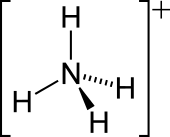
\includegraphics[scale = 0.5]{ammonium.png} \\ 
We first analyze a perfectly symmetrical ammonium molecule $[NH_4]^+$.
$$K_R = \frac{1}{2} \frac{L^2}{I}$$
$$\hat{H}_R = \frac{1}{2} \frac{\hat{L}^2}{I}$$
So we obtain the following eigen-equation:
$$\frac{1}{2} \frac{\hat{L}^2}{I} \psi = E_r \psi \implies E_r = \frac{1}{2I}\hslash^2 l(l+1)$$
Now we analyze the Ammonia molecule $NH_3$.
In this case we have not a scalar, but a tensor of inertia, which is a diagonal $3$x$3$ matrix, if we use the principles axis of inertia as our system of reference.\\ \\ 
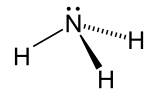
\includegraphics[scale = 0.5]{ammonia.png} \\  \\
In this case we get:
$$ \hat{H}_R = \frac{1}{2} \Biggl[ \frac{\hat{L}_x^2}{I_x} + \frac{\hat{L}_y^2}{I_y}+ \frac{\hat{L}_z^2}{I_z} \Biggl] = \frac{1}{2} \Biggl[ \frac{\hat{L}_x^2 + \hat{L}_y^2 + \hat{L}_z^2}{I_{xy}}- \frac{\hat{L}_z^2}{I_{xy}} + \frac{\hat{L}_z^2}{I_z} \Biggl] = \frac{1}{2} \Biggl[ \frac{\hat{L}^2}{I_{xy}} + \hat{L}_z^2 \Biggl( \frac{1}{I_z}- \frac{1}{I_{xy}} \biggl) \Biggl]
$$

$$\hat{H}_R \ket{l,m} = E_R(l,m) \ket{l,m} = E_R (l,m) \ket{l,m} = \frac{1}{2} \Biggl[ \frac{\hslash^2l(l+1)}{I_{xy}} + \hslash^2m^2 \biggl( \frac{1}{I_z} - \frac{1}{I_{xy}} \biggl) \Biggl] \ket{l,m}$$
In the case of the $CO_2$, we have a linear molecule.
\\ \\ 
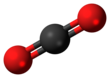
\includegraphics[scale = 1]{co2.png} $\hat{H}_R = \frac{1}{2} \frac{\hat{L}_x^2+ \hat{L}_y^2}{I_{xy}} \, \ E_R(l,m) = \frac{1}{2} \hslash^2 \frac{l(l+1)}{I_{xy}} \ $ 
\newpage
\textbf{Stern-Gerlach Experiment} \\ \\ 
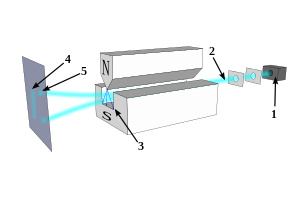
\includegraphics[scale = 0.7]{sge.png} \\ 
$$\hat{L}_z = -i \hslash \frac{\partial}{\partial \theta_z} \psi(\theta_z) = L_z \psi(\theta_z) \implies L_z = \hslash m, \ \psi(\theta_z) = c e^{im\theta_z}$$
We impose that:
$$\psi(\theta_z) = c e^{im\theta_z} = c e^{im(\theta_z+4\pi)}$$
For $2\pi = 0\pi$, the wave-function assumes two different values, so we must deal with a two-valued function.
So we will work in a tensor product space:
$$\mathcal{H}_r \otimes \mathcal{H}_s$$
We assume the $\begin{bmatrix} 1 \\ 0 \end{bmatrix}$ and $\begin{bmatrix} 0 \\ 1 \end{bmatrix}$ to be our basis vectors for the spin Hilbert space $\mathcal{H}_s$.
We define the operator $\hat{S}_z$.
We impose, following the results from the Stern-Gerlach experiment, that : 
$$\hat{S}_z \begin{bmatrix} 1 \\ 0 \end{bmatrix} = \frac{\hslash}{2} \begin{bmatrix} 1 \\ 0 \end{bmatrix}$$
$$\hat{S}_z \begin{bmatrix} 0 \\ 1 \end{bmatrix} = -\frac{\hslash}{2} \begin{bmatrix} 0 \\ 1 \end{bmatrix}$$
Thus:
$$\hat{S}_z = \frac{\hslash}{2} \begin{bmatrix}1 & 0 \\0 & 1 \end{bmatrix}
$$
Let's remember that $l = m_{MAX} = \frac{1}{2}$ and  we get:
$$\hat{S}^2  \begin{bmatrix} \alpha \\ \beta \end{bmatrix} = \hslash^2 \frac{1}{2} \biggl( \frac{1}{2} + 1 \biggl)   \begin{bmatrix} \alpha \\ \beta \end{bmatrix}  = \hslash^2 \frac{3}{4}  \begin{bmatrix} \alpha \\ \beta \end{bmatrix}$$
We can also define the $\hat{S}_+$ operator:
$$\hat{S}_+ \ket{s_z = \frac{\hslash}{2}} = 0$$
$$\hat{S}_+ \ket{ s_z = -\frac{\hslash}{2}} = c_+ \ket{s_z = -\frac{\hslash}{2}} = \hslash \sqrt{l(l+1)-m(m+1)} = \hslash \ket{s_z = \frac{\hslash}{2}}$$
Where  $m= -\frac{1}{2}$ and l = $\frac{1}{2}$.

\section{Lecture 19}

We impose the following conditions:
$$\hat{S}_+ \begin{bmatrix}
    1 \\ 0
\end{bmatrix} = \Vec{0}, \ \hat{S}_+ \begin{bmatrix}
    0 \\ 1
\end{bmatrix} = c_+ \begin{bmatrix}
    1 \\ 0
\end{bmatrix} = \hslash \begin{bmatrix}
    1 \\ 0
\end{bmatrix}  
$$
From the first condition it follows that:
$$\hat{S}_+ \begin{bmatrix}
    1 \\ 0
\end{bmatrix} = \begin{bmatrix}
    \alpha & \beta \\ \gamma & \delta \\
\end{bmatrix} \begin{bmatrix}
    1 \\ 0
\end{bmatrix}= \begin{bmatrix}
    0 \\ 0
\end{bmatrix} \implies \alpha = 0, \gamma = 0$$
From the second condition it follows that:
$$\hat{S}_+ \begin{bmatrix}
    0 \\ 1
\end{bmatrix} = \begin{bmatrix}
    0 & \beta \\ 0 & \delta \\
\end{bmatrix} \begin{bmatrix}
    0 \\ 1
\end{bmatrix}= \hslash \begin{bmatrix}
    1 \\ 0
\end{bmatrix} \implies \beta = \hslash, \delta = 0. $$
Thus we get that;
$$\hat{S}_+ = \hslash \begin{bmatrix}
    0 & 1 \\ 0 & 0 \\
\end{bmatrix}$$
In the same way, we obtain that:
$$ \hat{S}_- = \hslash \begin{bmatrix} 0 & 0 \\ 1 & 0 \\
\end{bmatrix}$$
We can now write the following system of equations: \\ 
$$
\begin{cases}
\hat{S}_+ = \hat{S}_x + i \hat{S}_y \\ 
\hat{S}_- = \hat{S_x} - i \hat{S}_y  
\end{cases} \implies \begin{cases}
\hat{S}_x = \frac{1}{2} (\hat{S}_+ + \hat{S}_-) \\ 
\hat{S}_y = -\frac{i}{2}(\hat{S}_+- \hat{S}_-) 
\end{cases} $$
We obtain the following two matrices:
$$\hat{S}_x = \frac{\hbar}{2} \begin{pmatrix} 0 & 1 \\ 1 & 0 \end{pmatrix} = \frac{1}{2} \hslash \hat{\sigma}_x$$
$$ \hat{S}_y = \frac{\hbar}{2} \begin{pmatrix} 0 & -i \\ i & 0 \end{pmatrix} =  \frac{1}{2} \hslash \hat{\sigma}_y$$

$$\hat{\Vec{S}}_{\vec{v}} = v_x \hat{S}_x+ v_y \hat{S}_y + v_z \hat{S}_z  $$
Now let's evaluate the following commutators:
$$ [ \hat{S}_x, \hat{S}_y ] = \hat{S}_x \hat{S}_y - \hat{S}_y\hat{S}_x= i\hslash \hat{S}_z$$
Similarly, we get:
$$[\hat{S}_y, \hat{S}_z] = i \hslash \hat{S}_x$$
$$[\hat{S}_z, \hat{S}_x] = i \hslash \hat{S}_y$$
We get results analogous to the ones that we obtain for the commutators for the $\hat{L}_{x/y/z}$ operators. For Fermions it holds stat:
$$ \hat{S}^2 = \hat{\Vec{S}}\hat{\Vec{S}}^* = \biggl( \frac{1}{2} \hslash \biggl)^2 \bigl( |\sigma_x^2|+ |\sigma_y|^2+ |\sigma_z|^2 \bigl) = \frac{3}{4} \hslash^2 \hat{I}$$
With $s = \frac{1}{2}$, we can write: $\hat{S}^2 = \hslash^2 s(s+1)\hat{I}$.
All the Fermions have spin $s=\frac{1}{2}$. Instead all the Bosons have spin $ s = 1$, save from the Higg's Boson which have spin $s=0$.
For a two atoms system, in the tensor product space, we can choose as a basis the following kets:
$$\ket{x_0, \uparrow}, \ket{x_0, \downarrow}, \ket{-x_0, \uparrow}, \ket{-x_0, \downarrow}$$ \\
$$\hat{\Vec{J}} = \hat{\Vec{L}}+ \hat{\Vec{S}}$$
$$\hat{S}_{TOT} = \hat{S}_1 + \hat{S}_2$$ \\ 
\textbf{Theorem: Addition of Angular Momentum}\\
If we have a composite systems, expressed by the two kets the allowed values of the total angular momentum quantum number $j_{TOT}$, given
two angular momenta corresponding to quantum numbers $j_1$ and $j_2$, are
$j_{TOT} = j_1 + j_2, j_1 + j_2 - 1, \cdots | j_1 - j_2 | $ and for each of these values of $j, m $ takes on the $(2j + 1)$ values
$m = j, j - 1, ... , -j$.
The proof of this theorem is beyond the scope of this course. \\ \\
Let's fix the following quantities, for $s= \pm \frac{1}{2}$:$$\hat{S}_{TOT} \ket{e_1,e_2} = \hslash^2 S_{TOT} (S_{TOT}+1) \ket{e_1,e_2}$$
$$0 \leq S_{TOT} \leq 1$$
There is a relation between $\hat{\Vec{\mu}}$ and $\hat{\Vec{S}}$ that can be expressed through the Bohr Magneton:
$$\hat{\Vec{\mu}} = \frac{g \mu_B}{\hslash} \hat{\Vec{S}}$$
$$\hat{H}_B = \hat{\Vec{\mu}}\Vec{B}$$
For the electron $g_e= 2$. We also get that:
$$\Vec{B}' = \frac{\Vec{V} \cross \Vec{E}}{c}$$
$$\hat{H}' = \hat{H} = \hat{\Vec{\mu_s}} \Vec{B}' = \hat{\Vec{\mu}}_s \frac{\Vec{V}\cross\Vec{E}}{c}$$\\
For a particle with spin 1, the spin matrices are the following ones:

$$
S_x = \frac{\hslash}{\sqrt{2}} \begin{bmatrix}
0 & 1 & 0 \\
1 & 0 & 1 \\
0 & 1 & 0
\end{bmatrix}
$$

$$
S_y = \frac{\hslash}{\sqrt{2}} \begin{bmatrix}
0 & -i & 0 \\
i & 0 & -i \\
0 & i & 0
\end{bmatrix}
$$

$$
S_z = \hslash \begin{bmatrix}
1 & 0 & 0 \\
0 & 0 & 0 \\
0 & 0 & -1
\end{bmatrix}
$$
$$S^2 = 2\hslash I$$

\section{Lecture 20}
\textbf{Identical Particles}
$$\psi(\Vec{r}_1, s_1,\Vec{r}_2,s_2),\ \psi(\Vec{r}_2,s_2,\Vec{r}_1,s_1)$$
$$\hat{H} = \hat{T}_k+ \hat{V}_ex(\Vec{r}_1) \hat{V}_ex(\Vec{r}_2)+ \hat{V}_{int}(|\Vec{r}_1-\Vec{r}_|,|s_1-s_2|)$$
Doing a permutations on two identical particle does not change the state of our quantum systems, thus we introduce the permutation operator:
$$\hat{P}_{12} = \hat{P}_{21} \implies \psi(\Vec{r}_1,s_1,\Vec{r}_2,s_2) = \hat{P}_{12}\psi(\Vec{r}_2,s_2,\vec{r}_1,s_1).$$
Since $\hat{P}^2 = \hat{I} $, we can conclude that its eigenvalues are $\pm 1.$ \\
We conclude that $\psi(\vec{r}_1,s_1,\vec{r}_2,s_2) = \pm \psi(\vec{r}_2,s_2,\vec{r}_1,s_1)$. \\
We now impose that changing the labels of the wave function representing a state, doesn't change its energy, thus:
$$\hat{H}\ket{\psi} = E\ket{\psi}$$
$$\implies \hat{H}\hat{P}\ket{\psi(x_1,x_2} = E\hat{P}\ket{\psi(x_2,x_1} = \hat{P}\hat{H}\ket{\psi(x_1,x_2)}$$
$$\implies [\hat{H},\hat{P}] = 0$$
From the Ehrenfest Theorem, we can conclude that If the system starts out in an eigenstate of $\hat{P}$ symmetric or antisymmetric, it will stay that way forever. \\ \\
Particle with eigenvalue $-1$ are the so called Fermions, antisymmetric particles, while particle with eigenvalue $1$ are the so called Bosons, which are symmetric particles.\\
Let's now consider two independent particle, whose wave function is the product of the wave functions:
$$\hat{H} \psi(\vec{r}_1,s_1,\vec{r}_2,s_2) = \bigl[ (\hat{T}_{k_1}+ \hat{V}_1) +(\hat{T}_{k_2}+ \hat{V}_2) \bigl] \psi(\vec{r}_1,s_1) \psi(\vec{r}_2,s_2) = E_{TOT}\psi_1(\vec{r}_1,s_1)\psi_2(\vec{r}_2,s_2) $$

$$ \implies \begin{cases}
     \hat{T}_{k_1}+ \hat{V}_1 = E_1\psi(\vec{r}_1,s_1) \\
     \hat{T}_{k_2}+ \hat{V}_2 = E_2\psi(\vec{r}_2,s_2) \\
\end{cases}$$
Thus we get that $E_{TOT} = E_1+ E_2$. \\
Now we will deduce the the Pauli Exclusion Principle, for two non interacting identical fermions in the ground state $0$, with same spin $s=s_1=s_2$ we get:
$$\psi = \psi_0(\vec{r}_1,s,\vec{r}_2,s)= \psi_0(\vec{r}_1,s)\psi_0(\vec{r}_2,s)= -\psi_0(\vec{r}_2,s,\vec{r}_1,s) = -  \psi_0(\vec{r}_2,s)\psi_0(\vec{r}_1,s)=0$$
Our framework is a two dimensional Hilbert space:
$$
\begin{cases}
\psi(\vec{r}_1)\ket{s_1}_1\\
\psi(\vec{r}_2)\ket{s_2}_2\\
\end{cases} \implies \psi(\vec{r}_1)\ket{s_1}_1\psi(\vec{r}_2)\ket{s_2}_2
$$
The product of the two functions satisfies the Schrodinger equation, but we must also impose to have an antisymmetric function. Thus:
$$f(x,y) = g(x,y)-g(y,x) = -f(y,x)$$
Since this is a linear combination of solutions to the Schrodinger Equation, it is still a solution, with the enforced constraint of being antisymmetric.
$$\frac{1}{\sqrt{2}}\bigl[\psi(\vec{r}_1)\ket{s_1}_1\psi(\vec{r}_2)\ket{s_2}_2-\psi(\vec{r}_2)\ket{s_2}_1\psi(\vec{r}_1)\ket{s_1}_2\bigl] = \frac{1}{\sqrt{2}}\psi(\vec{r}_1)\psi(\vec{r}_2) \bigl[ \ket{s_1}_1\ket{s_2}_2-\ket{s_2}_2\ket{s_1}_1 \bigl] = \star $$
If $s_1=s_2 \implies \star = 0 $.\\
We have have tried to obtain an antisymmetric solution to the Schrodinger Equation, by a linear combination of a solution, obtaining a null function which is not acceptable since it is not normalizable.\\
Let's consider Helium, which has two electrons:\\
$|s_1-s_2| \leq S_{TOT}  \leq |s_1+s_2| \implies 0  \leq S_{TOT}  \leq 1 $. \\ 
In the ground state, there are two electrons in the same orbitals, so for the Pauli Exclusion Principle they must have opposite spin. We have that:
\begin{itemize}
    \item $ S_{TOT}^2 \ket{0} = 0 $ for the ground singlet state.
\item $S_{TOT}^2 \ket{1} = \hslash \cdot 1 \cdot (1+1) \ket{1}$ for the triplet state.
\end{itemize}
We can now state the Pauli Exclusion Principle: Two electrons can't have the same state and same spin.

\section{Lecture 21}
The objective is to find a function for the fermions which is solution to the Schrodinger equation, and that has also the correct parity.
$$\psi_1(\vec{r}_1,s_1) = \frac{1}{\sqrt{v}}e^{i \Vec{k}_1 \Vec{r}_1} \ket{s_1}_1$$
$$\psi_2(\vec{r}_2,s_2) = \frac{1}{\sqrt{v}}e^{i \Vec{k}_2 \Vec{r}_2} \ket{s_2}_2$$
We are considering two non interacting particles:
$$\psi(\vec{r}_1,s_1,\vec{r}_2,s_2) = \frac{1}{\sqrt{2}v} \biggl( e^{i \Vec{k}_1 \Vec{r}_1}e^{i \Vec{k}_2 \Vec{r}_2} \ket{s_1}_1\ket{s_2}_2 \pm e^{i \Vec{k}_1 \Vec{r}_2}e^{i \Vec{k}_2 \Vec{r}_1}  \ket{s_2}_1 \ket{s_1}_2 \biggl)$$
$$\psi^*(\vec{r}_1,s_1,\vec{r}_2,s_2) = \frac{1}{\sqrt{2}v} \biggl( e^{-i \Vec{k}_1 \Vec{r}_1}e^{-i \Vec{k}_2 \Vec{r}_2} \bra{s_1}_1\bra{s_2}_2 \pm e^{-i \Vec{k}_1 \Vec{r}_2}e^{-i \Vec{k}_2 \Vec{r}_1} \bra{s_2}_1 \bra{s_1}_2 \biggl)$$
\begin{gather*}
    |\psi(\vec{r}_1,s_1,\vec{r}_2,s_2) |^2 = \frac{1}{2v^2} \Bigl[2 \pm e^{-i \Vec{k}_1 \Vec{r}_1} e^{-i \Vec{k}_2 \Vec{r}_2} e^{i \Vec{k}_1 \Vec{r}_2}e^{i \Vec{k}_2 \Vec{r}_1}\bra{s_1}_1\ket{s_2}_1 \bra{s_2}_2  \ket{s_1}_2 \pm \\ \pm e^{-i \Vec{k}_1 \Vec{r}_2}e^{-i \Vec{k}_2 \Vec{r}_1}e^{i \Vec{k}_1 \Vec{r}_1} e^{i \Vec{k}_2 \Vec{r}_2} \bra{s_2}_1\ket{s_1}_1 \bra{s_1}_2\ket{s_2}_2 \Bigl)
\end{gather*}
If $s_1=s_2$ we do the calculations, we get that:
\begin{gather*}
|\psi(\vec{r}_1,s_1,\vec{r}_2,s_2) |^2  = \frac{1}{2v^2} \Bigl[2 \pm e^{-i \Vec{k}_1 \Vec{r}_1} e^{-i \Vec{k}_2 \Vec{r}_2} e^{i \Vec{k}_1 \Vec{r}_2}e^{i \Vec{k}_2 \Vec{r}_1} \pm e^{-i \Vec{k}_1 \Vec{r}_2}e^{-i \Vec{k}_2 \Vec{r}_1}e^{i \Vec{k}_1 \Vec{r}_1} e^{i \Vec{k}_2 \Vec{r}_2} \Bigl]
\end{gather*}
\begin{gather*}
    |\psi(\vec{r}_1,s,\vec{r}_2,s)|^2 = \frac{1}{2v^2} \Bigl[2 \pm e^{i\vec{k}_1(\Vec{r}_2-\vec{r}_1)} e^{i\vec{k}_2(\Vec{r}_1-\vec{r}_2)} \pm e^{-i\vec{k}_1(\Vec{r}_2-\vec{r}_1)} e^{-i\vec{k}_2(\Vec{r}_1-\vec{r}_2) }  \Bigl]  \\ \implies |\psi(\vec{r}_1,s,\vec{r}_2,s)|^2 = \frac{1}{v^2} \biggl( 1 \pm cos\bigl( (\vec{k}_1-\vec{k}_2) \cdot (\vec{r}_1-\vec{r}_2) \bigl) \biggl)
\end{gather*}
If instead we have that $s_1 =s = -s_2$, we get:
$$|\psi(\vec{r}_1,s,\vec{r}_2,-s)|^2 =\frac{1}{2v^2} \Bigl[ 2 \pm 0 \pm 0 \Bigl]= \frac{1}{v^2}  $$
In one dimension, for a same spin system, and introducing as a coordinate for the difference of the wave vector, we can write that:
$$ |\psi|^2 = \frac{1}{v^2} \biggl( 1 + cos\bigl(k(x_1-x_2)\bigl)\biggl) $$

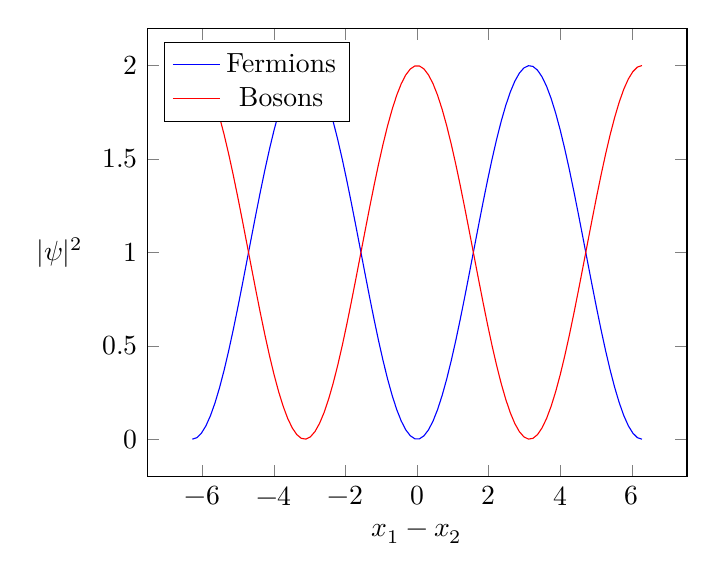
\begin{tikzpicture}
  \begin{axis}[
    xlabel={$x_1 - x_2$},
    ylabel={$|\psi|^2$},
    ylabel style={rotate=-90},
    domain=-2*pi:2*pi,
    samples=100,
    legend pos=north west
  ]
    \addplot[blue] {1 - cos(deg(x))};
    \addlegendentry{Fermions}
    \addplot[red] {1 + cos(deg(x))};
    \addlegendentry{Bosons}
  \end{axis}
\end{tikzpicture}
\\The probability density for fermions has a node at $(x_1-x_2) = 0$, which means that fermions cannot occupy the same position, consistent with the Pauli exclusion principle. On the other hand, the probability density for bosons is maximum at $(x_1-x_2) = 0$, indicating that bosons can occupy the same position.
\\ \\ 
\textbf{Entanglement}
$$\Phi^{\pm} = \frac{1}{\sqrt{2}} \Bigl( \psi_1(\vec(r)_1) \ket{\uparrow} \psi_2(\Vec{r}_2) \ket{\uparrow} \pm \psi_1(\vec{r}_1) \ket{\downarrow} \psi_2(\vec{r}_2) \ket{\downarrow} \Bigl)$$
$${\Phi^{\pm}}' = \frac{1}{\sqrt{2}} \Bigl( \psi_1'(\vec{r}_1) \ket{\uparrow} \psi_2'(\vec{r}_2) \ket{\downarrow} \pm \psi_1'(\vec{r}_1) \ket{\downarrow} \psi_2'(\vec{r}_2) \ket{\uparrow} \Bigr)$$
Entangled state means that you know some properties of the system, but  not about its components.
\section{Lecture 22}
The EPR paradox is a thought experiment that challenges the completeness and locality of quantum mechanics. It was proposed by Albert Einstein, Boris Podolsky and Nathan Rosen in 1935. \\
The paradox involves two particles that are entangled with each other, meaning that their quantum states are correlated even when they are separated by a large distance. According to quantum mechanics, each particle does not have a definite value for any observable (such as position or momentum) until it is measured. Instead, it exists in a superposition of possible values, with some probability for each outcome.\\ \\
The paradox arises when one of the particles is measured by an observer, say Alice. This measurement collapses the superposition and reveals a definite value for the observable. But at the same time, it also determines the value of the same observable for the other particle, which can be measured by another observer, say Bob. This means that Bob can predict with certainty the outcome of his measurement, without disturbing his particle in any way.\\ \\
Einstein, Podolsky and Rosen argued that this implies that there must be some hidden variables that determine the values of the observables for both particles before they are measured. These hidden variables would provide a more complete description of reality than quantum mechanics, which they considered incomplete. They also invoked a principle of locality, which states that no physical influence can travel faster than light. They reasoned that if there are no hidden variables, then quantum mechanics would violate locality, because the measurement by Alice would instantaneously affect the particle measured by Bob, at a speed faster than light.\\ \\ 
The EPR paradox has important implications for the interpretation of quantum mechanics and the nature of reality. It sparked a long debate between Einstein and Niels Bohr, who defended the Copenhagen interpretation of quantum mechanics and rejected the idea of hidden variables. It also inspired various experiments to test whether quantum mechanics violates locality or not. Following experiments have confirmed that the Copenhagen Interpretation was correct and ruled out certain types of hidden variables. \\ \\ 
The experiments ruled out the assumption of local-realism by Albert Einstein.
 \\ \textbf{Realism}: the value of an observable is not defined by measurement. The act of observation is not defining the reality, the result is predefined a-priory, and only discovered after the observation.
 \\ \textbf{Locality}: an object is directly influenced only by its immediate surroundings.  \\ \\
 Let's define the following wave function.
$$\psi^- = \frac{1}{\sqrt{2}} \Bigl( \ket{\uparrow^A_Z \downarrow^B_Z} - \ket{\downarrow^A_Z \uparrow^B_Z} \Bigl)$$
We define a correlation function, where $a,b$ identify two axis:
$$C(a,b) \triangleq \frac{S_a^A S_b^B}{h^2s^2}$$ \\
Without losing generality, we can assume the  $a$-axis to be equal to the $z$-axis, $a=z$.
\begin{gather*}
    \langle S_a^AS_b^B \rangle = \bra{\psi^-}\hat{S}_a^A\hat{S}_b^B \ket{\psi^-} = \frac{1}{2} \Bigl[ \bra{\uparrow^A_Z \downarrow^B_Z} \hat{S}_z^A\hat{S}_b^B \ket{\uparrow^A_Z \downarrow^B_Z}  + \bra{\downarrow^A_Z \uparrow^B_Z} \hat{S}_z^A\hat{S}_b^B \ket{\downarrow^A_Z \uparrow^B_Z} - \\  - \cancel{\bra{\uparrow^A_Z \downarrow^B_Z} \hat{S}_z^A\hat{S}_b^B \ket{\downarrow^A_Z \uparrow^B_Z} }-  \cancel{\bra{\downarrow^A_Z \uparrow^B_Z} \hat{S}_z^A\hat{S}_b^B \ket{\uparrow^A_Z \downarrow^B_Z}}  \Bigl] = \frac{1}{2} \Bigl[ \hslash s \bra{\downarrow_Z^B} \hat{S}_b^B \ket{\downarrow_Z^B} - \hslash s \bra{\uparrow_Z^B} \hat{S}_b^B \ket{\uparrow_Z^B} ] = \\ \frac{1}{2} \Bigl[ - \hslash s \bra{\uparrow_Z^B} \hat{S}_b^B \ket{\uparrow_Z^B} - \hslash s \bra{\uparrow_Z^B} \hat{S}_b^B \ket{\uparrow_Z^B} ] = - \hslash s \bra{\uparrow_Z^B} \hat{S}_b^B \ket{\uparrow_Z^B} = - \hslash s \bra{\uparrow_Z^B} \hat{S}_z^B \ket{\uparrow_Z^B}cos\theta_Z
\end{gather*}
\begin{enumerate} 
\item Write the expectation value of the product of spin operators $\hat{S}_a^A$ and $\hat{S}_b^B$ for two spin-1/2 particles A and B in the singlet state $\ket{\psi^-}$, which is an entangled state of opposite spins along any direction. \\ 
\item Expand the singlet state in terms of the eigenstates of $\hat{S}_z^A$ and $\hat{S}_z^B$, which are $\ket{\uparrow^A_Z \downarrow^B_Z}$ and $\ket{\downarrow^A_Z \uparrow^B_Z}$, with eigenvalues $\pm \hslash/2$ respectively. This is done by using the identity $$\ket{\psi^-} = \frac{1}{\sqrt{2}} \left( \ket{\uparrow^A_Z \downarrow^B_Z} - \ket{\downarrow^A_Z \uparrow^B_Z} \right)$$
 \item Apply the spin operators to the eigenstates and use the fact that they are diagonal in this basis, meaning that they only give non-zero results when acting on the same state. This allows us to cancel out two terms that involve cross-terms like $\bra{\uparrow^A_Z \downarrow^B_Z} \hat{S}_z^A\hat{S}_b^B \ket{\downarrow^A_Z \uparrow^B_Z}$, which are zero because $\bra{\uparrow^A_Z \downarrow^B_Z}$ and $\ket{\downarrow^A_Z \uparrow^B_Z}$ are orthogonal. We also use the fact that $$\hat{S}_z^A\ket{\uparrow^A_Z} = \frac{\hslash}{2}\ket{\uparrow^A_Z}$$ and $$\hat{S}_z^A\ket{\downarrow^A_Z} = -\frac{\hslash}{2}\ket{\downarrow^A_Z}$$
 \item Simplify the remaining terms by noting that we only need to consider the action of $\hat{S}_b^B$ on the states of particle B, since the states of particle A are already factored out. We also use the fact that $$\bra{\uparrow_Z}\hat{S}_b\ket{\uparrow_Z} = \bra{\uparrow_Z}\hat{S}_z\ket{\uparrow_Z}\cos\theta_b$$ where $\theta_b$ is the angle between the z-axis and the direction of $\hat{S}_b$. This follows from the rotation properties of spin operators and spinors. Similarly, we have $$\bra{\downarrow_Z}\hat{S}_b\ket{\downarrow_Z} = -\bra{\uparrow_Z}\hat{S}_b\ket{\uparrow_Z}$$
 \item  The final step is to combine the terms and obtain the final result, which is $$\langle S_a^AS_b^B \rangle = - \hslash s \bra{\uparrow_Z}\hat{S}_b\ket{\uparrow_Z}\cos\theta_b$$ where $s=1/2$ is the spin quantum number of each particle. This expression shows that the expectation value of the product of spin operators depends on the relative orientation of $\hat{S}_a$ and $\hat{S}_b$, and that it is always negative for the singlet state, meaning that the spins are anti-correlated.
 \end{enumerate}
The kets $\ket{\uparrow^A_Z \downarrow^B_Z}$, are eigenstate of $\hat{S}_z^A$, so they get multiplied by a constant, and are orthogonal to the bra operating on them, so we can cross out the two terms. Remember again that multiplying by $-1$ is the same of reverting the spin.
$$\langle S_a^AS_b^B \rangle =  - \hslash s \bra{\uparrow_Z^B} \hat{S}_z^B \ket{\uparrow_Z^B}cos\theta_Z = - \hslash^2 s^2 cos\theta_Z$$
$$\implies C(a,b) = \frac{\langle S_a^AS_b^B \rangle}{\hslash^2 s^2} = \frac{- \hslash^2 s^2 cos\theta_Z}{\hslash^2 s^2}= - cos\theta_Z$$
Now we will try to apply realism and locality assumptions:
$$\langle S_a^AS_b^B \rangle = \hslash^2s^2 \bigl[ P(S_a^A= S_b^B)-P(S_a^A=-S_b^B) \bigl] = \star $$
Since $P(S_a^A = S_b^B) + P(S_a^A = -S_b^B) =1$
$$\implies \langle S_a^A=S_b^B \rangle = \star = \hslash^2s^2\bigl[ 1-2P(S_a^A=-S_b^B)] \implies C(a,b) = 1-2P(S_a^A=S_b^B)$$
Now we will consider the measurements made by Alice, introducing another axis $c$. We define the following probability, and the correlation function as follows:
$$P(S_a^A=S_b^A)+P(S_a^A=S_c^A)+P(S_b^A=S_c^A) \geq 1$$
Due to the locality argument, and the independence of the measurements made by Alice and Bob, we must conclude that:
$$P(S_a^A=-S_b^B) = P(S_a^A=S_b^A)$$
$$P(S_a^A=-S_c^B) = P(S_a^A=S_c^A)$$
$$P(S_b^A=-S_c^B) = P(S_b^A=S_c^A)$$

$$C(a,b) = 1-2P(S_a^A=-S_b^B)$$
$$C(a,c) = 1-2P(S_a^A=-S_c^B)$$
$$C(b,c) = 1-2P(S_b^A=-S_c^B)$$
\textbf{Bell Inequality}
$$C(a,b)+C(a,c)+C(b,c) = 3-2\bigl[ P(S_a^A=-S_b^B)+P(S_a^A=-S_c^B) + P(S_b^A=-S_c^B) \bigl] =  $$
$$= 3 -2 \bigl[ P(S_a^A=S_b^A)+P(S_a^A=S_c^A)+P(S_b^A=S_c^A)  \bigl] \leq 1$$
Changing the sign of one the detectors/axis, makes us measure the opposite correlation function. We start by considering the opposite of the $c$ axis.
$$C(a,b)+C(a,-c)+C(b,-c) \leq 1$$
$$C(a,b)-C(a,c)-C(b,+c) \leq 1$$
$$C(a,b)-C(a,c) \leq 1+ C(b,c)$$
Now we will proceed by inverting the $a$ axis:
$$C(-a,b)-C(-a,c) \leq 1 + C(b,c)$$
$$-C(a,b)+C(a,c) \leq 1 + C(b,c)$$
$$ C(a,b)-C(a,c) \geq - \bigl(1+ C(b,c)\bigl)$$
$$\implies | C(a,b)-C(a,c) | \leq 1+ C(b,c) $$
Let $\theta_{ab} = \frac{\pi}{2}, \theta_{ac} = \frac{\pi}{4}, \theta_{bc} = \frac{\pi}{4}$:
$$C(a,b) = -cos(\theta_{ab})$$
$$C(a,b) = 0$$
$$C(a,c) = -\frac{\sqrt{2}}{2}$$
$$C(a,c) = -\frac{\sqrt{2}}{2}$$\\
This choice of angles, obviously violate the Bell Inequality.\\ \\
\textbf{Experimental Bell Tests}\\ \\
The first Bell test experiment was performed in 1972 by John Clauser and Stuart Freedman. It was designed to test whether quantum mechanics violates local realism, which is the assumption that physical reality is independent of observation and that no influence can travel faster than light. The experiment involved measuring the polarization of pairs of photons that were entangled, meaning that their quantum states were correlated even when they were separated in space. The experiment used a device called a polarizer to measure the polarization of each photon along a chosen direction. The experimenters varied the directions of the polarizers randomly and compared the results of the measurements. They found that the correlations between the photons were stronger than what any local hidden variable theory could explain, thus violating Bell’s inequality. This was the first experimental evidence that quantum mechanics predicts nonlocal phenomena that cannot be accounted for by classical physics.
The modification by Alain Aspect in his Bell test experiment was to use variable polarizers that could be changed randomly and rapidly during the measurements. This was done to close the locality loophole, which is the possibility that the entangled particles could somehow influence the settings of the polarizers and thus create a false impression of nonlocality. Aspect used an acousto-optic modulator to switch the orientation of the polarizers at a frequency of 50 kHz, which was much faster than the time it took for light to travel between the two measurement stations. This ensured that the polarizer settings were truly independent and unpredictable, and that no signal could travel from one station to another in time to affect the outcome. Aspect's experiment confirmed the violation of Bell's inequality with high statistical significance, and ruled out any local hidden variable theory.\\ \\
\textbf{Hidden Variables}\\ \\
The Hidden variable assumption is that $S_{a}^A = S_a^A(\xi),S_b^A = S_b^A(\xi),S_c^A = S_c^A(\xi) $ and that $S_a^B = -S_a^A(\xi),S_b^B = -S_b^A(\xi),S_c^B = -S_c^A(\xi)$, where $\xi$ is the hidden variable, which explains the measurement results "a priori".
$$\langle S_a^AS_b^B \rangle = \int f(\xi)S_a^A(\xi)S_b^B(\xi) d\xi = -\int f(\xi)S_a^A(\xi)S_b^A(\xi)d\xi$$
\begin{gather**}
\langle S_a^AS_b^B \rangle - \langle S_a^AS_c^B \rangle = - \int f(\xi) \bigl[ S_a^A(\xi)S_b^A(\xi)-S_a^A(\xi)S_c^A(\xi)\bigl]d\xi = \\  = - \int f(\xi)S_a^A(\xi)S_b^A(\xi) \biggl[1-\frac{1}{\hslash^2s^2}S_b^A(\xi)S_c^A(\xi)\biggl] d\xi
\end{gather**} \\ \\
Knowing that $\bigl( S_a^A \bigl)^2 = \hslash^2 s^2$. \\
\begin{gather**}
 \bigl| \langle S_a^AS_b^B \rangle - \langle S_a^AS_c^B \rangle \bigl| \leq \int f(\xi) \bigl| S_a^A(\xi)S_b^A(\xi) \bigl| \biggl[1-\frac{1}{\hslash^2s^2}S_b^A(\xi)S_c^A(\xi)\biggl] d\xi \leq \\ \leq \hslash^2 s^2\int f(\xi) \biggl[ 1-\frac{1}{\hslash^2 s^2}S_b^A(\xi)S_c^A(\xi) \biggl] d\xi
\end{gather**} \\ \\
The term $1-\frac{1}{\hslash^2 s^2}S_b^A(\xi)S_c^A(\xi)$ is outside the absolute value because it represents an adjustment factor applied to the absolute value of $S_a^A(\xi)S_b^B(\xi)$. This adjustment factor accounts for the relationship between the measurements $S_b^A(\xi)$ and $S_c^A(\xi)$.
To determine if we can assume this term is always positive, let's analyze the expression:
$$1-\frac{1}{\hslash^2 s^2}S_b^A(\xi)S_c^A(\xi)$$
Recall that $(S_a^A)^2 = \hslash^2 s^2$, which means that $S_a^A(\xi)$ is limited in magnitude by $\hslash s$. Similarly, $S_b^A(\xi)$ and $S_c^A(\xi)$ will also be limited in magnitude by $\hslash s$. 
Now, consider the product $S_b^A(\xi)S_c^A(\xi)$. Given that both factors are limited in magnitude by $\hslash s$, their product will be limited in magnitude by $(\hslash s)^2 = \hslash^2 s^2$ (CS-Inequality). 
When we divide the product by $\hslash^2 s^2$, the result will be limited in magnitude by 1:
$$\frac{1}{\hslash^2 s^2}S_b^A(\xi)S_c^A(\xi) \leq 1$$
Finally, subtracting this term from 1, we get:
$$1-\frac{1}{\hslash^2 s^2}S_b^A(\xi)S_c^A(\xi) \geq 0$$
Since the term is always non-negative, it does not affect the sign of the absolute value of $S_a^A(\xi)S_b^B(\xi)$. \\
Therefore, we can safely assume that the term $1-\frac{1}{\hslash^2 s^2}S_b^A(\xi)S_c^A(\xi)$ is always non-negative, and it is appropriate to place it outside the absolute value.\\ \\
Since $f(\xi)$ is a probability density function, its integral over the whole space is equal to 1.
$$\bigl| \langle S_a^AS_b^B \rangle - \langle S_a^AS_c^B \rangle  \bigl| \leq  \hslash^2s^2 -  \langle S_b^AS_c^A \rangle =  \hslash^2s^2  + \langle S_b^AS_c^B \rangle  $$
$$|C(a,b) -C(a,c)| \leq 1 +C(b,c)$$
There are not hidden variables. Quantities are defined by measurements.



\end{document}


